\documentclass[11pt,letterpaper]{article}

\usepackage[margin=1in]{geometry}
\usepackage{lmodern}
\usepackage[T1]{fontenc}
\usepackage[utf8]{inputenc}
\usepackage{microtype}
\usepackage{amsmath,amssymb,amsthm,mathtools}
\usepackage{graphicx}
\usepackage{booktabs}
\usepackage{tabularx}
\usepackage{caption}
\usepackage{xcolor}
\usepackage{fancyhdr}
\usepackage{xr-hyper}
\usepackage{hyperref}
\externaldocument[S-]{Paper1_JEDC_online_supplement}
\graphicspath{{../paper1_core/}{../paper1_note/}}

\definecolor{jedcblue}{RGB}{24, 62, 114}
\hypersetup{
  colorlinks=true,
  linkcolor=jedcblue,
  citecolor=jedcblue,
  urlcolor=jedcblue,
  pdftitle={Observationally Equivalent Algorithms: What Prices Reveal About Trader Populations, and What Supervisors Need},
  pdfauthor={Pratik Niroula, Prashant Niroula, Sujan Khatiwada}
}

\setlength{\parskip}{2.5pt plus 1pt minus 1pt}
\setlength{\parindent}{1.2em}
\linespread{1.03}
\emergencystretch=3em

\pagestyle{fancy}
\fancyhf{}
\fancyhead[L]{\small\scshape Niroula, Niroula, and Khatiwada}
\fancyhead[R]{\small\scshape Observationally Equivalent Algorithms}
\fancyfoot[C]{\small\thepage}
\renewcommand{\headrulewidth}{0.4pt}

\fancypagestyle{plain}{
  \fancyhf{}
  \fancyfoot[C]{\small\thepage}
  \renewcommand{\headrulewidth}{0pt}
}

\newtheorem{theorem}{Theorem}[section]
\newtheorem{proposition}[theorem]{Proposition}
\newtheorem{corollary}[theorem]{Corollary}
\newtheorem{lemma}[theorem]{Lemma}
\theoremstyle{definition}
\newtheorem{remark}[theorem]{Remark}
\newtheorem{definition}[theorem]{Definition}

\newcommand{\E}{\mathbb{E}}
\newcommand{\R}{\mathbb{R}}
\newcommand{\KL}{\mathrm{KL}}
\newcommand{\TV}{\mathrm{TV}}
\newcommand{\Var}{\mathrm{Var}}
\newcommand{\supp}{\mathrm{supp}}

\begin{document}
\hypersetup{pageanchor=false}
\thispagestyle{empty}
\begin{center}
  {\LARGE\bfseries Observationally Equivalent Algorithms:\\[4pt]
  What Prices Reveal About Trader Populations,\\[4pt]
  and What Supervisors Need\par}
  \vspace{1.2em}
  {\large Pratik Niroula\footnote{Department of Computer Information Science, Minnesota State University, Mankato, MN 56001, USA. Email: \texttt{pratik.niroula@mnsu.edu}.} \qquad
  Prashant Niroula\footnote{Faculty of Management, Tribhuvan University, Kirtipur, Nepal. Email: \texttt{prashantniroula20@gmail.com}.} \qquad
  Sujan Khatiwada\footnote{Department of Electrical, Computer and Robotics Engineering, Minnesota State University, Mankato, MN 56001, USA. Email: \texttt{sujan.khatiwada@mnsu.edu}.}}
  \vspace{0.8em}

  {\normalsize November 2026}
\end{center}

\vspace{0.6em}
\begin{abstract}
\noindent
We study markets in which heterogeneous trading algorithms feed a common public pricing signal back into order flow. In a linear market and in a stationary inventory-dealer equilibrium, every public outcome depends on the trader population only through its aggregate feedback kernel. Within one passive record of pricing errors this yields a supervisory separation. With impact and persistence held fixed, whether a uniform feedback cut meets a stability ceiling depends only on the aggregate budget, which the record estimates at a near-parametric rate however close the traders' memories are. In the dealer equilibrium the cut moves impact and persistence; on the principal equilibrium branch it still lowers the budget, and its size is learned at a slower rate that again does not depend on the spacing of memories. Whether a targeted restriction meets the ceiling can require of order $\Delta^{-(4K-2)}$ observations when $K$ classes have memory rates within $\Delta$; verified class tags, or a pilot of the restriction, remove that penalty. Cheap relabeling erodes tags, and against a fixed untagged test traders gain by crowding their memories. Class-tagged flows from the Taiwan Stock Exchange illustrate the magnitudes.
\end{abstract}

\vspace{0.5em}
\noindent\textbf{Keywords:} algorithmic trading; feedback trading; aggregate response; observational equivalence; market supervision; disclosure.\\
\noindent\textbf{JEL Classification:} C32, D83, G14, G18.\\
\noindent\textbf{Online Supplement and Replication:} References of the form ``Supplement Theorem~S4.1'' are to the Online Supplement, which states every result in full; the full working paper (Niroula et al., 2026d) collects further results on the feedback model. Technical lemmas, extended proofs and numerical checks are in the Online Supplement. Lean~4 formalizations check the deterministic steps and several finite-sample probability bounds; asymptotic steps are proved on paper. Supplement Table~\ref{S-tab:claims} records, for every main-text result, whether it is proved in Lean from Mathlib, proved in Lean under stated hypotheses, or proved on paper only. The replication archive is \url{https://github.com/Pratikn03/Fianince} (version of 28 November 2026). Extensions to breach cascades, strategic insiders, and nonlinear or learning traders appear in a companion note (Niroula et al., 2026c).

\newpage
\hypersetup{pageanchor=true}
\setcounter{page}{1}

\section{Introduction}

A market supervisor can often measure how strongly a market reacts to its own past prices long before it can say which traders produce that reaction. The two are different objects. If a policy scales every trader group's feedback by the same factor, the aggregate response is all the supervisor needs to evaluate it. If the policy halts one class of traders, the supervisor needs that class's own contribution. This paper asks where the line between the two falls, and what it costs a supervisor to cross it.

The mechanism is easiest to see with two algorithms. Suppose each trades on an exponentially weighted average of past pricing errors, one with memory rate $0.49$ and the other with $0.51$, in equal size. Prices clear only aggregate order flow, so the two blend: together they produce nearly the same flow as a single group at $0.50$. The first-order difference cancels, the second lag tap differs by order $\Delta^2$ with $\Delta = 0.01$, and detecting the difference takes of order $\Delta^{-4}$ noisy observations. Populations of two groups each can be matched more closely: pairs that agree through the second moment differ at order $\Delta^3$ and need of order $\Delta^{-6}$ observations, and with $K$ nearby groups on each side the requirement is $\Delta^{-(4K-2)}$. A uniform cut does not care about this blending. A targeted halt does.

\textbf{The model.} We put heterogeneous feedback-trading algorithms into a linear market and into an inventory-dealer equilibrium. With a common public signal and fixed causal rules, the trader population enters every public outcome---prices, total order flow, insider profits and dealer inventories---only through its aggregate flow map (Theorem~\ref{n:suff}). For linear rules this map is the \emph{feedback kernel}, the moment sequence of the population's merged memory-rate measure. In Section~\ref{sec:equilibrium}, price impact comes from competitive, risk-averse dealers who carry inventory, and the persistence of pricing errors from the share of inventory they carry overnight, which we take as given. Dealers observe the pricing error, and the equilibrium depends on the population only through the merged measure, the one population object they need. Equilibrium prices follow the same closed-loop recursion with unchanged memory rates (Theorems~\ref{n:thm_inventory} and~\ref{n:thm_eqreduced}), so the identification barriers below are equilibrium properties, not artifacts of mechanical price impact; Theorem~\ref{n:eqcut} takes the uniform cut into the same equilibrium.

\textbf{The main result.} Theorem~\ref{n:separation} is a supervisory separation stated inside one experiment. In one passive record of pricing errors, given persistence, impact and a memory bound, whether a uniform feedback cut meets a stability ceiling depends on the population only through the aggregate budget, which the record estimates at a near-parametric rate however close the traders' memories are (Theorem~\ref{n:passiveupper}); whether a targeted restriction meets the same ceiling can require of order $(\Delta\eta)^{-(4K-2)}$ observations of the same record (Proposition~\ref{n:target}). The same separation holds for reset probes, where verified class tags also remove the spacing penalty for class weights (Theorem~\ref{n:disc}), and without tags the uniform cut is minimax over labelings (Theorem~\ref{n:minimax}). Theorem~\ref{n:eqcut} takes the uniform cut into the dealer equilibrium, where the cut moves impact and persistence. The post-cut budget then depends on the population through the Stieltjes transform of the merged measure at the new dealer root, so the fixed-impact formula is wrong in size and, on a lower equilibrium branch, in sign. On the principal branch a cut lowers the budget, populations that prices cannot tell apart end within $(\Delta\eta)^{2K-1}$ of each other, and one passive record estimates the post-cut budget at a polynomial rate that does not depend on the spacing. A pilot of a targeted restriction removes the penalty after the fact: the pilot record identifies the post-restriction budget directly, and the change in the price response identifies the removed groups' kernel, exactly when impact is fixed and after a correction fixed by the two dealer roots in equilibrium (Theorem~\ref{n:pilot}).

\textbf{The limits of tags.} Tags work only as long as traders cannot game them. If restricted traders can route activity through accounts carrying another label at convex cost $\gamma$, the optimal restriction is partial and class tags lose all value as $\gamma \to 0$ (Proposition~\ref{n:relabel}). Records that link accounts to beneficial owners keep their value only to the extent that they make such routing visible; the model takes this as a property of the audit trail, not as a result. Without tags, surveillance invites a different response. Against a fixed-level test whose power grows at least like the square root of the divergence, a high-stakes untagged algorithm moves its memory toward its neighbor as the supervisor's record $N$ grows. Divergence scales as $N\delta^4$ in the memory distance $\delta$, so the supervisor's information falls at rate $N^{-1}$ and detection collapses toward the false-alarm rate (Theorem~\ref{n:paradox}). This is the group's best response to a fixed test, not an equilibrium with an optimizing supervisor; a two-sided test, whose power rises with the divergence rather than its square root, slows the crowding. A longer price record therefore does not substitute for an owner-linked one: against a group that best-responds to a one-sided test, the price record's value is at most of order $N^{-1/2}$, and at most of order $N^{-1/6}$ against a two-sided test (Theorem~\ref{n:recordvalue}).

\textbf{Supporting results.} Theorem~\ref{n:cost} proves the barrier for passive observation and for active impulse probes. It extends to smooth causal rule families and is matched by Prony and minimum-distance recovery (Supplement Theorems~\ref{S-n:univ} and~\ref{S-n:shape}), and it does not vanish as the market approaches instability (Supplement Proposition~\ref{S-prop:nearcrit}; Figure~\ref{fig:near-instability}). Market-wide linear functionals of the merged measure, such as discounted feedback or single-lag taps, are estimated at the parametric rate $\sigma^2\epsilon^{-2}$ whatever the spacing (Theorem~\ref{n:questions} and Corollary~\ref{n:sep}). In a Gaussian feedback market, the Kullback--Leibler divergence between two candidate populations equals half the cumulative excess forecast MSE divided by the innovation variance (Theorem~\ref{n:dual}): composition does not matter for forecasting prices, only for attributing them. Smooth quadratic trading charges can be evaluated from passive pricing-error records, while proportional taxes, exit thresholds and binding turnover caps cannot (Supplement Proposition~\ref{S-thm:instruments}), and with verified partial tags, policies uniform within each tagged group are minimax (Supplement Theorem~\ref{S-n:minimaxtags}).

\textbf{What is new, and what is not.} The minimax rate $\Delta^{-(4K-2)}$ is the known rate for finite mixtures with near-colliding components (Heinrich and Kahn, 2018; Wu and Yang, 2020) and for super-resolution of point sources (Batenkov et al., 2021), and the modulus characterization of linear functionals builds on Donoho (1994). We do not claim those results. Three statistical results adapt known tools to the closed loop. Theorem~\ref{n:passiveupper} feeds a long autoregression (Berk, 1974) into Prony's method. Its closest relatives are single-path estimation of the distribution of autoregressive coefficients from autocovariances (Leipus et al., 2006; Celov et al., 2010) and non-asymptotic identification of linear systems from one trajectory (Simchowitz et al., 2018; Oymak and Ozay, 2019; Sarkar et al., 2021); what the feedback market adds is that the autoregressive coefficients are the kernel taps and that positivity bounds the spectrum uniformly in the population, so the tap error does not depend on the spacing. Supplement Proposition~\ref{S-prop:nearcrit} is a near-unit-root statement: matched budgets make the composition difference vanish at zero frequency, so, as in the near-unit-root asymptotics of Chan and Wei (1988) and Sims et al.\ (1990), information about directions other than the long-run one stays bounded. Theorem~\ref{n:pilot} is a corollary of Theorem~\ref{n:cost}(iii) once a restriction deletes part of the population. That market-wide policies need only a reduced-form aggregate while targeted ones need structure is Marschak's maxim and the logic of sufficient statistics for policy (Marschak, 1953; Chetty, 2009). What we add is the informational price of that structure in a feedback market and its equilibrium form: kernel sufficiency survives inventory-equilibrium pricing, in which dealer anticipation over-weights slow memories; in that equilibrium the reduced form a market-wide cut needs is more than the aggregate budget, yet it is still learned without the spacing penalty (Theorem~\ref{n:eqcut}); uniform rules are minimax over labelings; and tags have strategic limits, both from relabeling and from crowding.

\textbf{Empirical illustration.} Daily class-tagged institutional order flows from the Taiwan Stock Exchange (300 stocks, 2013--2016) illustrate the model's magnitudes (Section~\ref{sec:taiwan}). At daily frequency the feedback share is small. With impact and non-feedback flow granted, the price-consistent effect of halting foreign feedback ranges from zero to the whole uniform effect. The exercise is an illustration, not a test: the persistence it displays is largely produced by the detrending filter, the tags identify class contributions only under the restriction that feedback memory equals flow persistence, and a registered out-of-sample test of the feedback premise does not separate feedback from prices revealing past flow.

\subsection{Related literature}

\textbf{Aggregation and observational equivalence.} Exponential memory is classical in dynamic economics, spanning adaptive expectations (Cagan, 1956; Nerlove, 1958), geometric distributed lags (Koyck, 1954), and steady-state Kalman filtering (Muth, 1960). That aggregate dynamics depend only on a distribution of micro coefficients dates back to Granger (1980), Forni and Lippi (1997), Zaffaroni (2004), and Pesaran and Chudik (2014), with recovery of the cross-sectional distribution forming the disaggregation problem (Celov et al., 2010). Observational equivalence in policy evaluation traces to Sargent (1976) and, for sufficient statistics in heterogeneous-agent macroeconomics, Auclert et al.\ (2024). A large literature studies heterogeneous fundamentalist and chartist asset-pricing models (Brock and Hommes, 1998; Hommes, 2006) and estimates trader shares from prices (Boswijk et al., 2007; Franke and Westerhoff, 2012; Lux and Zwinkels, 2018): whereas Brock and Hommes model fitness-driven predictor switching and Heinrich and Kahn study i.i.d.\ mixture sampling, we hold rules and masses fixed so composition enters through the moments of a single measure observed via a closed-loop feedback recursion. Our results establish precisely which features of a trader population are recoverable from prices and at what statistical cost. Feedback traders are central to models of destabilizing speculation and of return autocorrelation (De Long et al., 1990; Cutler et al., 1990; Sentana and Wadhwani, 1992), and simulation-based estimation of agent-based models (Grazzini and Richiardi, 2015; Platt, 2020) faces the same identification question in nonlinear models. Our identification result is global (Theorem~\ref{n:ident}); where memories collide, the information matrix of Rothenberg (1971) is singular, and Theorem~\ref{n:cost} and Supplement Theorem~\ref{S-n:shape} give the rate at which identification weakens near a collision. Our minimax results are decisions under ambiguity in the sense of Manski (2000). Our decision-theoretic framing connects Blackwell (1953) and Le Cam (1964) with data-driven control (van Waarde et al., 2020) and aggregate forecasting (L\"utkepohl, 1987; Hendry and Hubrich, 2011).

\textbf{Microstructure, trader identity, and algorithmic supervision.} Prior microstructure studies show that broker or trader identity carries price-discovery information when order flow reflects private fundamentals (Frino et al., 2010; Linnainmaa and Saar, 2012), while Sanders et al.\ (2009) document weak predictive content of large-trader positions in agricultural futures. Our setting isolates a distinct mechanism: under a common public signal, identity is irrelevant for price discovery and forecasting, yet essential for assigning targeted supervisory interventions. Inventory-based price impact goes back to Ho and Stoll (1981) and Grossman and Miller (1988), and Hendershott and Menkveld (2014) measure it. Crowding among algorithmic and quantitative strategies is documented by Chaboud et al.\ (2014) and Khandani and Lo (2011) and analyzed by Stein (2009); pre-trade anonymity in limit-order markets, which concerns who quotes rather than who trades on feedback, is studied by Foucault et al.\ (2007). In regulatory policy, Budish et al.\ (2015) analyze continuous-book cancellation and batch auctions, while Colliard and Hoffmann (2017) document volume, liquidity, and composition responses to a transaction tax (complementing our fixed-memory scheduled-holding benchmark in Supplement Proposition~\ref{S-thm:instruments}), Kirilenko et al.\ (2017) use account-level audit-trail data to reconstruct the Flash Crash, and Menkveld (2016) surveys high-frequency trading. SEC Rule~613 established the Consolidated Audit Trail (CAT) to link orders to customer identities across venues (Securities and Exchange Commission, 2012). Our disclosure game---building on costly state falsification (Lacker and Weinberg, 1989; Crocker and Morgan, 1998)---provides a formal rationale for that architecture: market-wide remedies require only prices, targeted restrictions require class records, and cheap relabeling favors owner-linked audit trails. Acting on market information can degrade it (Bond et al., 2010; Bond and Goldstein, 2015), and manipulation muddles the signals a principal relies on (Frankel and Kartik, 2019, 2022; Perez-Richet and Skreta, 2022).

\textbf{Roadmap.} Section~\ref{sec:model} presents the baseline model and unified notation. Section~\ref{sec:sufficiency} establishes kernel sufficiency and noiseless identification. Section~\ref{sec:equilibrium} derives price impact and persistence in an inventory equilibrium and proves that all identification results carry over. Section~\ref{sec:cost} quantifies the sample complexity of composition versus market-wide questions. Section~\ref{n:irr_sec} equates pairwise detection with forecast mismatch. Section~\ref{sec:supervision} analyzes the separation, the uniform cut in equilibrium, minimax policy, disclosure, relabeling, the surveillance paradox, and the Taiwan illustration. Section~\ref{sec:conclusion} discusses scope and concludes. Appendix~\ref{app:proofs} proves the headline results (Theorems~\ref{n:suff}, \ref{thm:what-id}, \ref{n:passiveupper}, \ref{n:separation}, \ref{n:eqcut} and~\ref{n:pilot}); the other proofs are in Supplement Section~\ref{S-app:proofs}.

\section{Model and Notation}\label{sec:model}

Time is discrete, $t = 0, 1, 2, \dots$. In theoretical Sections~\ref{sec:model}--\ref{sec:supervision}, let $p_t$ and $F_t$ denote dollar prices and fundamental value per share, and $x_t = p_t - F_t$ the dollar pricing error per share (making CARA-normal linear demand exact across long and short positions; empirical log-price proxies $\log P_t$ are reserved for Section~\ref{sec:taiwan}). In the reduced-form benchmark, a dealer sector absorbs net order flow with price impact $\kappa > 0$, and arbitrage pulls the pricing error toward zero with persistence $a \in [0, 1)$. (Section~\ref{sec:equilibrium} derives both $a$ and $\kappa$ endogenously from competitive inventory-averse dealers.)

There are $K \ge 1$ groups of feedback traders with adaptation rates $\eta_i \in (0, 1)$ and activity weights $q_i$. Group $i$ maintains an exponentially weighted average $y_{i,t}$ of past pricing errors and submits feedback flow $q_i y_{i,t}$:
\begin{equation}\label{eq:baseline}
  x_t = a x_{t-1} + \kappa \sum_{i=1}^K q_i y_{i,t-1} + \kappa v_t + \varepsilon_t,
  \qquad
  y_{i,t} = (1 - \eta_i) y_{i,t-1} + \eta_i x_t,
\end{equation}
where $v_t$ is an observer's executed probe trade (with $v_t \equiv 0$ under passive observation) and $\varepsilon_t$ is a price innovation (news). As shown in Supplement Lemma~\ref{S-lem:micro}, both a trading desk tracking a latent random-walk trend via a steady-state Kalman filter (Muth, 1960) and a desk updating via $L_2$-regularized online gradient descent satisfy the exact recursion in~\eqref{eq:baseline}.

Write $r_i = 1 - \eta_i \in (0, 1)$ for group $i$'s \emph{memory rate} and $w_i = q_i \eta_i$ for its \emph{merged trading weight}. Define the \emph{merged measure} $M = \sum_{i=1}^K w_i \delta_{r_i}$, which sums weights over any groups sharing an identical memory rate. The \emph{feedback kernel} is the sequence of power moments of $M$:
\begin{equation}\label{eq:kernel}
  k_m = \sum_{i=1}^K w_i r_i^m = \int r^m \, dM(r), \qquad m = 0, 1, 2, \dots
\end{equation}
Total feedback flow is the causal convolution of past pricing errors with $k$. Define the \emph{feedback budget}
\begin{equation}\label{eq:budget}
  S = a + \kappa \sum_{i=1}^K q_i = a + \kappa \sum_{m=0}^\infty k_m.
\end{equation}
In the positive-feedback economy ($q_i \ge 0$), the closed-loop system~\eqref{eq:baseline} is Schur stable if and only if $S < 1$; when $S \ge 1$, no stationary equilibrium exists and inventory variance diverges. With contrarian groups ($q_i < 0$), $S < 1$ rules out a unit root at $\omega = 0$, $\sup_\omega |L(e^{i\omega})| < 1$ for $L(e^{i\omega}) = e^{-i\omega}(a + \kappa \sum_{m \ge 0} k_m e^{-i\omega m})$ gives a sufficient small-gain test, and necessary and sufficient Schur stability holds by the Nyquist criterion for $L(e^{i\omega})$ around $+1$ (all roots of $1 - z(a + \kappa \sum_{m\ge 0} k_m z^m) = 0$ outside $|z| \le 1$, Supplement Section~\ref{S-sec:mixed_sign}). Table~\ref{tab:notation} summarizes our unified notation across sections.

\begin{table}[!htbp]
\centering
\caption{Summary of core notation across sections.}
\label{tab:notation}
\small
\begin{tabularx}{\linewidth}{@{}lX@{}}
\toprule
Symbol & Economic meaning \\
\midrule
$x_t, F_t, p_t$ & Dollar pricing error ($x_t = p_t - F_t$), fundamental, and price (log proxy in Sec.~\ref{sec:taiwan}) \\
$a, \kappa$ & Pricing-error persistence ($a \in [0,1)$) and price impact ($\kappa > 0$) \\
$\eta_i, r_i, q_i, w_i$ & Group $i$ adaptation rate, memory rate ($r_i = 1-\eta_i$), activity weight, merged weight ($w_i = q_i \eta_i$) \\
$M, S_M(D), G(z)$ & Merged measure $\sum_i w_i \delta_{r_i}$, Stieltjes transform $\sum_i w_i/(D - r_i)$, transfer $G(z) = \sum_i w_i z/(z - r_i)$ \\
$S, \bar{s}$ & Feedback budget $S = a + \kappa \sum_i q_i$ and prudential ceiling $\bar{s} \in (a, 1)$ \\
$H_t, \bar{a}, A$ & Dealer inventory, dealer carry share, and CARA risk aversion (Section~\ref{sec:equilibrium}) \\
$\Delta, \Delta\eta$ & Spread (half-width) of trader type parameters or memory rates around center $r_c$ \\
$u_d, U, \theta_c$ & Class $d$ feedback contribution ($u_d = \kappa q_d$), total feedback $U = \sum_d u_d$, policy scale $\theta_c$ \\
$\theta_{\mathcal{B}}, \theta_{\mathcal{H}}, \gamma, \alpha_{\mathcal{H}}$ & Retention rates for benign ($\mathcal{B}$) and harmful ($\mathcal{H}$) labels, relabeling cost $\gamma$, harm $\alpha_{\mathcal{H}} = -n_{\mathcal{H}}$ \\
$\delta, \delta_0, n, J$ & Distance to the neighbor's memory, preferred distance, divergence exponent ($n = 4$), divergence $J = cN\delta^n$ \\
\bottomrule
\end{tabularx}
\end{table}

\textbf{Observation regimes and the role of impact.} In the reduced-form identification analysis, the observer knows $(a, \kappa)$ and the noise law and observes $x_t$ (or a public signal from which $x_t$ is reconstructible). Giving the observer known $(a, \kappa)$ and exact observability of $x_t$ only strengthens the observer; hence all sample-complexity lower bounds hold \emph{a fortiori} when $(a, \kappa)$ must be estimated or when only raw transaction prices $p_t = F_t + x_t$ are observed with hidden fundamentals (Remark~\ref{rem:obs}). We analyze both passive price observation ($v_t = 0$) and active probing from a reset state. Reset probing is strictly an information-theoretic benchmark---not a proposed regulatory policy, as unscheduled exploratory order injection on live venues is constrained by anti-manipulation and anti-spoofing statutes (15 U.S.C.\ \S\,78i; MAR Art.\ 12)---demonstrating that even an idealized probing observer cannot escape the $\Delta^{-(4K-2)}$ barrier. Finally, mechanical impact in~\eqref{eq:baseline} describes limit-order-book mechanics or inventory-averse dealers (Section~\ref{sec:equilibrium}); by contrast, a risk-neutral market maker who knows the aggregate flow rule would net out predictable feedback flow, so prices would reveal \emph{less}, not more, about the population (no result here uses this; Niroula et al., 2026c, Proposition~C2.1(iv), states it formally).

\section{Kernel Sufficiency and Identification}\label{sec:sufficiency}

To establish sufficiency in full generality, embed the feedback population in a strategic market. An asset value $v$ is drawn, noise traders submit orders $z_t$, a strategic insider submits orders $X_t(v, \mathcal{H}_{t-1})$, and a dealer sets prices $P_t(\mathcal{H}_{t-1}, Y_t)$ from public history $\mathcal{H}_{t-1}$ and total order flow $Y_t = X_t + z_t + f_t$. Feedback groups update on a public signal $s_t = \mathcal{S}_t(p_0, \dots, p_t)$ and contribute aggregate flow $f_t = \sum_{m < t} k_m s_{t-1-m}$. The maps $X$, $P$, and $\mathcal{S}$ are arbitrary causal rules. The strategic players are the insider and the dealer; feedback-group rules are fixed, and their individual payoffs are not part of the payoff equivalence.

\begin{theorem}[The kernel is sufficient]\label{n:suff}
If two feedback-group configurations satisfy $k_m = k'_m$ for all $m < T$, then for every strategy profile $(X, P)$ and every realization of $(v, z)$, the price path, total order-flow path, insider trades and realized profit, and dealer inventory coincide on all dates $t \le T$. For games that end by date $T$, the two games share identical strategy sets and payoff functions, and hence identical equilibria under any solution concept defined from public histories and payoffs; with equal kernels at every lag the statement holds for every horizon. The same holds for any finite population whose individual flows are causal linear functions of the public signal, with $k$ the sum of individual kernels. Group-level quantities, such as the weight of the largest group, are not invariant.
\end{theorem}

The proof is a short induction on dates (Appendix~\ref{app:proofs}). Its economic force lies in the object it isolates: a single population-level sequence $k$ settles every equilibrium concept simultaneously. Because the induction uses only that aggregate feedback flow is a fixed causal map of public signals, sufficiency extends to arbitrary nonlinear or profit-switching populations via the aggregate flow map (Supplement Section~\ref{S-sec:suff}). Moreover, equal kernels remain observationally equivalent even when anonymous aggregate order flow is added to the public record.

The converse holds under the mechanical-impact observation experiment of Section~\ref{sec:model}:

\begin{theorem}[What prices identify]\label{n:ident}\label{thm:what-id}
In model~\eqref{eq:baseline}, fix known $(a, \kappa)$, $x_{-1} = 0$, and zero initial group states, and compare noiseless probe responses (Supplement Section~\ref{S-sec:suff}). Two economies produce identical price responses to every probe sequence if and only if their merged measures $M$ coincide.
\end{theorem}

Together, Theorems~\ref{n:suff} and~\ref{n:ident} establish that the feedback kernel (equivalently, the merged measure $M$, which has finitely many atoms) is a \emph{minimal identifying functional} of the trader population for prices: it determines everything prices can reveal, and noiseless prices determine it.

\section{Sufficiency and Identification in Inventory Equilibrium}\label{sec:equilibrium}

Section~\ref{sec:sufficiency} took price impact $\kappa$ and persistence $a$ as primitives. We now derive both in equilibrium from competitive, risk-averse dealers who take the overnight carry share $\bar{a} \in [0, 1)$ as given (passive capital absorbs $(1-\bar{a})H_{t-1}$ at the start of date $t$ while generation-$t$ dealers hold $H_t$ into $t+1$, with spreads or convex trading fees ruling out round-trip manipulation, Huberman and Stanzl, 2004; Supplement Section~\ref{S-sec:mixed_sign}), proving that kernel sufficiency and the $(\Delta\eta)^{-(4K-2)}$ identification barrier hold in equilibrium.

\textbf{The inventory economy.} Consider an infinite-horizon discrete-time market:
\begin{itemize}
  \item \emph{Fundamental and price.} The asset's fundamental value $F_t$ follows a public random walk with i.i.d.\ innovations of variance $\sigma_F^2$. The transaction price is $p_t = F_t + x_t$, where $x_t$ is the equilibrium pricing error induced by dealer inventory absorption.
  \item \emph{Feedback groups.} Group $i$ submits orders $u_{i,t+1} = r_i u_{i,t} + w_i x_t$, with memory rates $r_i = 1 - \eta_i \in (0, 1)$ and merged weights $w_i = q_i \eta_i$.
  \item \emph{Exogenous flow.} Total customer order flow is $Y_t = \sum_{i=1}^K u_{i,t} + \xi_t$, where fundamental innovations $\Delta F_t \sim N(0, \sigma_F^2)$ and exogenous flow shocks $\xi_t \sim N(0, \sigma_\xi^2)$ are mutually independent.
  \item \emph{Competitive dealers.} Overlapping generations of dealers with CARA risk aversion $A > 0$ absorb customer flow and exogenously carry fraction $\bar{a} \in [0, 1)$ of inventory overnight while passive off-market capital absorbs $(1 - \bar{a})H_{t-1}$ at the start of date $t$, so aggregate dealer inventory evolves as $H_t = \bar{a} H_{t-1} - Y_t$. Market clearing requires $H_t = (\E_t[p_{t+1}] - p_t)/(A V)$, where $V = \Var_t(p_{t+1})$ is the one-step conditional price variance.
\end{itemize}
Let $S_M(D) = \sum_{i=1}^K w_i / (D - r_i) = \int (D - r)^{-1} \, dM(r)$ denote the Stieltjes transform of the merged measure $M$ (distinct from $G(z)$ in frequency space).

\begin{theorem}[Price impact and persistence in inventory equilibrium]\label{n:thm_inventory}
Consider stationary linear equilibria in which $x_t$ is linear in dealer inventory $H_t$ and next-period feedback trades $\{u_{i,t+1}\}$.
\begin{enumerate}
  \item[(i)] \emph{Characterization.} The pricing law
  \[
    x_t = -\kappa H_t + \kappa \sum_{i=1}^K \frac{u_{i,t+1}}{D - r_i}, \qquad D \neq 0, \; D \neq r_i,
  \]
  is an equilibrium if and only if the induced state dynamics are Schur stable and $(\kappa, D, V)$ solve
  \begin{equation}\label{eq:eq-system}
    D = 1 - \kappa S_M(D), \qquad \kappa(D - \bar{a}) = A V D, \qquad V = \sigma_F^2 + \frac{\kappa^2 \sigma_\xi^2}{D^2}.
  \end{equation}
  An unexpected unit of order flow moves the price by $\kappa / D$.
  \item[(ii)] \emph{No-feedback benchmark.} When $w_i = 0$, $D = 1$ and $x_t = \bar{a} x_{t-1} + \kappa Y_t$. Persistence equals the dealer carry share $\bar{a}$, and impact solves $\kappa(1 - \bar{a}) = A(\sigma_F^2 + \kappa^2 \sigma_\xi^2)$. An equilibrium exists if and only if $\Lambda_0 \equiv (1 - \bar{a})^2 - 4 A^2 \sigma_F^2 \sigma_\xi^2 \ge 0$; when $\Lambda_0 > 0$, the low-impact root $\kappa_- \approx A \sigma_F^2 / (1 - \bar{a})$ is the equilibrium price of inventory risk.
  \item[(iii)] \emph{Invariance.} The equilibrium tuple $(\kappa, D, V)$ and the resulting price process depend on the trader population solely through $S_M$, and hence solely through the merged measure $M$.
  \item[(iv)] \emph{Small feedback.} Let $\Lambda_0 > 0$, fix $\delta > 0$ with $\max_i r_i < 1 - \delta$, and suppose $\epsilon = \sup_{|D - 1| \le \delta}(|S_M(D)| + |S_M'(D)|)$ is small. Then there exists a unique equilibrium near $(\kappa_-, 1)$, and with the aggregate feedback intensity $S_M(1) = \sum_i q_i$,
  \[
    D = 1 - \kappa_- S_M(1) + o(\epsilon), \qquad
    \kappa = \kappa_- + \frac{\kappa_-^2(\bar{a} + 2 A \kappa_- \sigma_\xi^2)}{\sqrt{\Lambda_0}}\, S_M(1) + o(\epsilon).
  \]
  Positive feedback increases both equilibrium price impact $\kappa$ and unexpected shock impact $\kappa / D$.
\end{enumerate}
\end{theorem}

\begin{remark}[Observability of pricing errors]\label{rem:obs}
Dealers and feedback traders in Theorem~\ref{n:thm_inventory} observe $x_t = p_t - F_t$ because $F_t$ is public among market participants while inventory-induced mispricing $x_t$ is earned by risk-averse dealers. An outside supervisor who observes only raw transaction prices $p_t = F_t + x_t$ without observing the random-walk fundamental $F_t$ receives strictly less information. Every sample-complexity lower bound derived below therefore holds \emph{a fortiori} under unobserved fundamentals (while Supplement Corollary~\ref{S-cor:unknown_primitives} shows that unknown primitives do not alter the upper-bound rate under active probes). The positive results, identification and the upper bounds, assume that the pricing error is observed.
\end{remark}

\begin{remark}[Mispricing feedback versus raw-return feedback]\label{rem:returns}
Theorem~\ref{n:thm_inventory} specifies feedback rules on the pricing error $x_t = p_t - F_t$, which isolates pure inventory-driven feedback in closed form. If algorithmic traders instead condition on raw price changes $\Delta p_t = \Delta F_t + \Delta x_t$, fundamental innovations $\Delta F_t$ enter the traders' memory states directly alongside inventory shocks. This introduces a second exogenous innovation channel. It does not alter pathwise kernel sufficiency (Theorem~\ref{n:suff}), which allows any public signal, and the lower bound of Supplement Theorem~\ref{S-n:univ}, which allows any smooth causal rule of the observed history, still applies when the observed innovations are Gaussian.
\end{remark}

Before turning to identification, we characterize how endogenous dealer risk-bearing alters stability as feedback scales up---replacing the linear $S \uparrow 1$ variance blow-up with a saddle-node liquidity fold at strictly finite variance:

\begin{theorem}[Equilibrium fragility and liquidity collapse]\label{thm:fragility}
Let $A, \sigma_F^2, \sigma_\xi^2 > 0$, $\bar{a} \in [0, 1)$, and $w_i > 0$ with $\Lambda_0 = (1 - \bar{a})^2 - 4 A^2 \sigma_F^2 \sigma_\xi^2 > 0$, holding intraday dealer risk tolerance $A^{-1}$ fixed. Write $S_M(D) = \sum_{i=1}^K w_i/(D - r_i)$ and scale feedback intensity by $\lambda S_M(D)$ for $\lambda \ge 0$. On the principal monotone branch $D \in (\max(D_{\min}, \max_i r_i), 1]$, where $D_{\min} \equiv \bar{a} + 2 A \sigma_F \sigma_\xi$:
\begin{enumerate}
  \item[(i)] \emph{Principal critical threshold and saddle-node exit.} There exists a finite threshold $\lambda_{\mathrm{crit}} \in \bigl(0, [\kappa_- S_M(1)]^{-1}\bigr)$ such that a stable linear equilibrium $(\kappa(\lambda), D(\lambda), V(\lambda))$ exists on the principal branch for $\lambda < \lambda_{\mathrm{crit}}$, whereas for $\lambda > \lambda_{\mathrm{crit}}$ no real equilibrium exists on $(\max(D_{\min}, \max_i r_i), 1]$ at fixed $A$.
  \item[(ii)] \emph{Liquidity collapse and square-root fragility.} Under the non-degenerate quadratic fold condition $F_{DD}(D_{\mathrm{crit}}; \lambda_{\mathrm{crit}}) > 0$ on $F_-(D; \lambda) \equiv D - 1 + \lambda \kappa_-(D) S_M(D)$, which we assume, as $\lambda \uparrow \lambda_{\mathrm{crit}}$, $D(\lambda) - D_{\mathrm{crit}} \asymp \sqrt{\lambda_{\mathrm{crit}} - \lambda}$ and effective depth $D/\kappa$ shrinks with square-root fold asymptotics.
  \item[(iii)] \emph{Finite threshold variance and diverging sensitivities.} At $\lambda = \lambda_{\mathrm{crit}}$ with $D_{\mathrm{crit}} > \max(D_{\min}, \max_i r_i)$ and $F_{DD} > 0$, conditional variance $V(\lambda_{\mathrm{crit}}) < 2\sigma_F^2 < \infty$, the effective closed-loop budget $S^*(\lambda_{\mathrm{crit}}) < 1$, and $\Var(H_t) < \infty$ remain strictly finite, while sensitivities $d\kappa/d\lambda$, $dV/d\lambda$, and $d\Var(H_t)/d\lambda$ diverge as $(\lambda_{\mathrm{crit}} - \lambda)^{-1/2} \to +\infty$ as $\lambda \uparrow \lambda_{\mathrm{crit}}$.
\end{enumerate}
\end{theorem}

The interval $(\max(D_{\min}, \max_i r_i), 1]$ can hold more than one root: with the primitives of Supplement Theorem~\ref{S-thm:eqreduced}(iv) both $D = 0.80$ and $D = 0.862$ are equilibria. We call the largest root the principal equilibrium; it is the one reached continuously from the no-feedback equilibrium as feedback is scaled up, and Theorem~\ref{n:eqcut} shows that comparative statics reverse on a root below it. For $K \ge 2$ with $\max_i r_i > D_{\min}$, further inter-pole branches may exist on $(D_{\min}, \max_i r_i)$, while long-run dealer entry unfolds the fixed-$A$ cliff into a smooth schedule (Supplement Section~\ref{S-sec:mixed_sign} and Figure~\ref{S-fig:supp_fragility}).

\begin{theorem}[Identification results carry over to equilibrium]\label{n:thm_eqreduced}
In any stationary equilibrium of Theorem~\ref{n:thm_inventory} with $D \neq \bar{a}$:
\begin{enumerate}
  \item[(i)] \emph{Exact reduced form.} Path by path, the equilibrium pricing error follows the closed loop~\eqref{eq:baseline} with effective persistence $a^* = \bar{a}/D$, effective impact $\kappa^* = \kappa/D$, unchanged memory rates $r_i$, and rescaled merged weights $\tilde{w}_i = w_i (D - \bar{a})/(D - r_i)$.
  \item[(ii)] \emph{Transmission zeros.} If $\bar{a} > 0$, the memory rates $r_i \in (0,1)$ are distinct, and weights $w_i > 0$, the $r_i$ remain the exact transmission zeros of the equilibrium price response.
  \item[(iii)] \emph{Identification boundary.} The effective merged measure $\tilde{M} = h M$, where $h(r) = (D - \bar{a})/(D - r)$ is positive whenever $D > \max_i r_i$, is in one-to-one correspondence with the primitive merged measure $M$. Thus $M$ remains the exact identifying functional of equilibrium prices.
  \item[(iv)] \emph{Minimax rate preservation.} Under the uniform stability condition $a^* + \kappa^* W / (1 - r_c - \Delta\eta) < 1$ of Theorem~\ref{n:cost}, two inventory equilibria with identical primitives $(A, \sigma_F^2, \sigma_\xi^2, \bar{a})$ that differ only in their feedback-trader composition form a pair requiring $N \ge c \sigma^2 (\Delta\eta)^{-(4K-2)}$ reset experiments to distinguish, each recording the equilibrium price response to a probe with Gaussian noise of variance $\sigma^2$.
\end{enumerate}
\end{theorem}

Part~(iv) uses the reset contract of Section~\ref{sec:cost}, a benchmark for what data can reveal rather than a description of a running market; the finite-record bound in the proof of Theorem~\ref{n:cost} gives the same order for one passive record. With the primitives of its realization both equilibrium roots satisfy part~(iv) (Supplement Section~\ref{S-sec:eqcut}). The proofs of Theorems~\ref{n:thm_inventory} and~\ref{n:thm_eqreduced} are given in Supplement Section~\ref{S-app:proofs}. Economically, forward-looking dealers anticipate predictable feedback trades and incorporate them into current quotes; rather than obscuring the memory rates, anticipation leaves $r_i$ untouched and up-weights slower-memory groups by $(D - \bar{a})/(D - r_i)$.

To organize the decision-theoretic consequences of sufficiency, we state the following immediate corollary of Blackwell (1953) and Le Cam (1964):

\begin{proposition}[What an intervention requires]\label{n:interv}
Suppose supervisory observations depend on the trader population only through its aggregate flow map.
\begin{enumerate}
  \item[(i)] If the observation law identifies the flow map and the loss depends on the population only through that map, the set of safe actions is identified in that experiment.
  \item[(ii)] If two populations share the same flow map and an action is safe in one but unsafe in the other, every observation-based rule takes that action with identical probability in both.
  \item[(iii)] If the observation laws of two populations lie within total-variation distance $\delta$, any rule that takes the action with probability $p$ where it is safe takes it with probability at least $p - \delta$ where it is unsafe.
\end{enumerate}
\end{proposition}

\section{The Sample-Complexity Price of Composition}\label{sec:cost}

Theorem~\ref{n:ident} establishes that groups with distinct memory rates are identifiable in principle. We now quantify how much data identification actually requires when memory rates are closely spaced, comparing passive price observation against the active-probing benchmark.

\begin{theorem}[The cost of composition]\label{n:cost}
Fix $K \ge 2$, a center memory rate $r_c \in (0,1)$, total merged weight $W > 0$, and small $\Delta\eta>0$ with $r_c+\Delta\eta[-1,1]\subset(0,1)$. Fix known $(a,\kappa)$ with $a+\kappa W/(1-r_c-\Delta\eta)$ bounded below one by a common positive margin over the spacings considered.
\begin{enumerate}
  \item[(i)] \emph{Passive price observation.} When prices are observed passively as the stationary output of~\eqref{eq:baseline} driven by i.i.d.\ Gaussian news $\varepsilon_t \sim N(0, \sigma^2)$, there exist two $K$-group economies with rates in $r_c + \Delta\eta[-1,1]$ and positive weights whose merged measures match all moments of order $0, \dots, 2K-2$, and whose Kullback--Leibler divergence per observation is of exact order $(\Delta\eta)^{4K-2}$. Distinguishing them with both error probabilities below $1/4$ requires $T \ge c (\Delta\eta)^{-(4K-2)}$ passive observations.
  \item[(ii)] \emph{Active probing is no cheaper.} Even if the supervisor can run $N$ independent reset experiments recording the noisy impulse response with Gaussian observation noise of variance $\sigma^2$, the same pair has impulse-response gap $O((\Delta\eta)^{2K-1})$, of that exact order when the lag-$2K$ impulse-response coefficient ("tap") $h_{2K}$ is recorded, requiring $N \ge c \sigma^2 (\Delta\eta)^{-(4K-2)}$ experiments.
  \item[(iii)] \emph{Matching upper bound.} On any compact class of $\gamma$-separated rescaled rates with weights bounded away from zero, Prony's method applied to the first $2K$ kernel values reconstructed from impulse responses through $h_{2K}$ attains fixed positive accuracy at fixed confidence with $O(\sigma^2(\Delta\eta)^{-(4K-2)})$ reset experiments, matching the lower bound on parameter families containing the hard pair.
\end{enumerate}
\end{theorem}

Supplement Section~\ref{S-app:proofs} gives the argument. Supplement Theorems~\ref{S-prop:passive}, \ref{S-thm:kcohort} and~\ref{S-prop:esprit} give further details. The hard pair consists of the $K$-point Gauss--Legendre and Gauss--Radau quadrature rules scaled to $r_c + \Delta\eta[-1,1]$, which match all moments through degree $2K-2$ while differing at order $2K-1$. For two groups ($K=2$), halving the memory spread multiplies the required data by $2^6 = 64$; for three groups ($K=3$), by $2^{10} = 1{,}024$. A global quadratic bound on the location KL of a news law can give the same lower-bound order in a sequential Gaussian-style comparison with common observed initialization and a uniform moment bound. The constant then uses that global bound.

\textbf{One passive pricing-error record attains the rates.} The upper bound in Theorem~\ref{n:cost}(iii) uses reset experiments. A single stationary record of pricing errors suffices too, because feedback flow is a causal filter of past pricing errors: with $v_t \equiv 0$, \eqref{eq:baseline} reads $x_t - a x_{t-1} = \kappa \sum_{j \ge 0} k_j x_{t-1-j} + \varepsilon_t$, an autoregression of infinite order whose coefficients are the kernel taps.

\begin{theorem}[One passive pricing-error record attains the rates]\label{n:passiveupper}
Fix known $(a, \kappa)$ with $a \ge 0$, $\kappa > 0$, and a margin $m \in (0, 1)$. Consider positive economies ($w_i \ge 0$) with budget $S \le 1 - m$, memory rates at most $\bar r < 1$ and total merged weight at most $\bar W$, observed through one stationary record $x_{1-L}, \dots, x_T$ of~\eqref{eq:baseline} with $v_t \equiv 0$ and i.i.d.\ $N(0, \sigma^2)$ news. Let $\hat\theta \in \R^L$ be the least-squares coefficients of $x_t - a x_{t-1}$ on $(x_{t-1}, \dots, x_{t-L})$, $\hat k = \hat\theta / \kappa$ and $\hat S = a + \sum_{j < L} \hat\theta_j$. For $\beta \in (0, 1/3)$ and $T \ge 128 L^2 / (m^4 \beta)$, with probability at least $1 - 3\beta$,
\[
  \|\hat k - (k_0, \dots, k_{L-1})\|_2 \le \frac{8\sqrt{L}}{\kappa}\Bigl(\frac{1}{m\sqrt{T\beta}} + \frac{\rho_L}{m^2 \beta}\Bigr),
  \qquad \rho_L = \frac{\kappa \bar W \bar r^L}{1 - \bar r},
\]
and $|\hat S - S| \le \kappa\sqrt{L}\, \|\hat k - (k_0, \dots, k_{L-1})\|_2 + \rho_L$. The news variance $\sigma^2$ does not enter.
\begin{enumerate}
  \item[(i)] \emph{The budget.} With $L$ of order $\log(1/(\epsilon\beta))$, $|\hat S - S| \le \epsilon$ with probability at least $1 - 3\beta$ once $T \ge C \epsilon^{-2} \beta^{-1} \log^2(1/(\epsilon\beta))$, whatever the number of groups and the spacing of their memories.
  \item[(ii)] \emph{Composition.} On the compact class of Theorem~\ref{n:cost}(iii) (rates $r_c + \Delta\eta\, s$ with $s$ $\gamma$-separated, weights in $[w_{\min}, w_{\max}]$, $w_{\min} > 0$, spacing $\Delta\eta \le \Delta\eta_0$), Prony's method applied to $\hat k_0, \dots, \hat k_{2K-1}$ recovers every weight to accuracy $\epsilon \in (0, \epsilon_0]$ with probability at least $1 - 3\beta$ once $L$ is of order $\log(1/(\epsilon\beta\Delta\eta))$ and
  \[
    T \ge C \epsilon^{-2} \beta^{-1} (\Delta\eta)^{-(4K-2)} \log\frac{1}{\epsilon\beta\Delta\eta}.
  \]
\end{enumerate}
The constants $C$ and $\epsilon_0$ depend only on $(\kappa, m, \bar r, \bar W)$ and, in~(ii), on $K$, $r_c$, $\Delta\eta_0$ and the class; through the threshold $T \ge 128 L^2/(m^4\beta)$, $C$ is of order $m^{-4}$ in the stability margin.
\end{theorem}

With Theorem~\ref{n:cost}(i), part~(ii) gives the passive sample requirement for composition, $(\Delta\eta)^{-(4K-2)}$ up to a logarithmic factor, from the record a supervisor actually has. Part~(i) does the same for the uniform cut: given $(a, \kappa)$, its budget is learned from passive prices at a near-parametric rate. The first step is the classical long autoregression (Berk, 1974); what the feedback market adds is that the autoregressive coefficients are the kernel taps, that positivity bounds the spectral density away from zero and infinity uniformly in the population, and that the tap error therefore does not depend on the spacing. In a simulation of a two-group economy from one stationary record ($a = 0.1$, $\kappa = 1$, $r_c = 0.45$, total weight $0.2$, memory offsets $\pm 0.5\,\Delta\eta$, $30$ lags, $40$ replications; replication archive), tap errors are flat in the spacing (fitted slope $-0.04$) and fall like $T^{-0.42}$, and weight errors have fitted slopes $-2.5$ in $\log\Delta\eta$ over $\Delta\eta \in [0.36, 0.70]$ and $-0.45$ in $\log T$. These spacings are far from the collision regime, so the simulation illustrates the estimator; it does not test the asymptotic exponent $-3$.

\textbf{The barrier does not lift near instability.} One might conjecture that as a market approaches instability ($S \uparrow 1$), feedback amplification magnifies compositional differences and makes traders easier to distinguish. It does so only boundedly. Give the hard pair of Theorem~\ref{n:cost} a common persistence and, by rescaling one economy's weights by a factor $1 + O((\Delta\eta)^{2K-1})$, a common feedback budget $S = 1 - \epsilon$. The passive KL divergence per observation then remains bounded by $C(\Delta\eta)^{4K-2}$ uniformly in $\epsilon > 0$ (Supplement Proposition~\ref{S-prop:nearcrit}): the gain from approaching instability is bounded and the exponent is unchanged. In Table~\ref{tab:years} the required years fall by factors of $1.35$ to $2.3$ as $1 - S$ falls from $0.1$ to $10^{-6}$. As Figure~\ref{fig:near-instability} illustrates, a market near instability reveals how close it is to instability, not who is trading in it. Table~\ref{tab:years} translates these lower bounds into illustrative calendar years of daily price data.

\begin{figure}[!htbp]
  \centering
  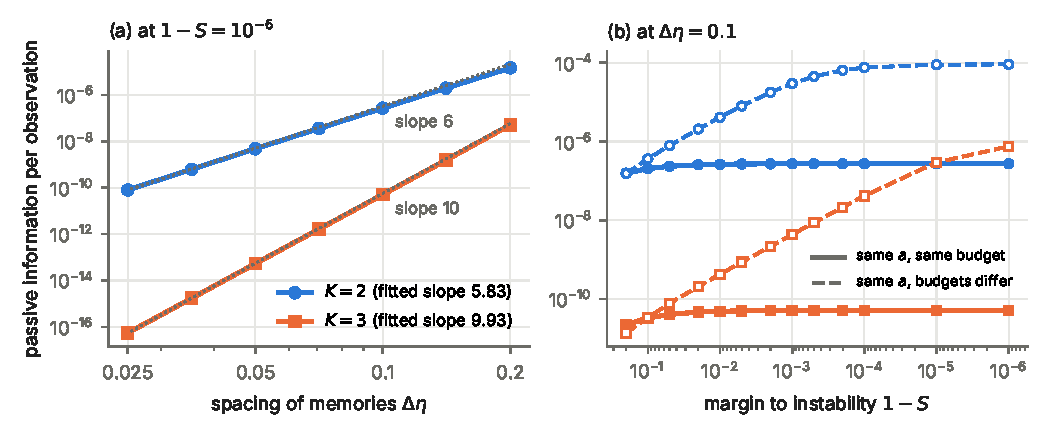
\includegraphics[width=\linewidth]{fig_barrier_admissible.pdf}
  \caption{The passive identification barrier near instability. Both panels plot the Gaussian Kullback--Leibler divergence per observation between the stationary price processes of the $K$-node Gauss and Gauss--Radau populations spread over $\Delta\eta$ around $r_c = 0.5$ (total weight $0.3$, impact $\kappa = 0.5$). Panel~(a): at a common persistence and a common feedback budget $1 - S = 10^{-6}$, information decays as $(\Delta\eta)^{4K-2}$ (fitted slopes $5.8$ and $9.9$). Panel~(b): with a common persistence and a common budget (solid; the Gauss--Radau weights rescaled by a factor $1 + O((\Delta\eta)^{2K-1})$), information stays bounded as $1 - S \to 0$. With a common persistence and no rescaling (dashed), the budgets differ by order $(\Delta\eta)^{2K-1}$; the information then grows roughly like $(1 - S)^{-1}$ until the margin reaches that gap, and levels off. Computed from the closed-form spectra; the code is in the replication archive.}
  \label{fig:near-instability}
\end{figure}

\begin{table}[!htbp]
\centering
\caption{Illustrative calendar years of daily price data required at $5\%$ per error, computed from the stationary KL rate of the budget-matched populations.}
\label{tab:years}
\small
\begin{tabular}{@{}llccc@{}}
\toprule
Groups & Memory rates & Half-lives (days) & Years ($1 - S = 0.1$) & Years ($1 - S = 10^{-6}$) \\
\midrule
$K = 2$ & $0.5 \pm 0.1$   & $0.8\text{--}1.4$  & $31{,}000$        & $23{,}000$ \\
        & $0.5 \pm 0.05$  & $0.9\text{--}1.2$  & $1.8 \times 10^6$ & $1.3 \times 10^6$ \\
        & $0.8 \pm 0.1$   & $1.9\text{--}6.6$  & $280$             & $160$ \\
        & $0.8 \pm 0.05$  & $2.4\text{--}4.3$  & $15{,}000$        & $8{,}100$ \\
        & $0.9 \pm 0.05$  & $4.3\text{--}13.5$ & $480$             & $230$ \\
        & $0.9 \pm 0.025$ & $5.2\text{--}8.9$  & $25{,}000$        & $11{,}000$ \\
\midrule
$K = 3$ & $0.5 \pm 0.1$   & $0.8\text{--}1.4$  & $2.0 \times 10^8$ & $1.3 \times 10^8$ \\
        & $0.5 \pm 0.05$  & $0.9\text{--}1.2$  & $1.9 \times 10^{11}$ & $1.2 \times 10^{11}$ \\
\bottomrule
\end{tabular}
\vspace{4pt}
\parbox{\linewidth}{\footnotesize\emph{Notes:} Rate-based proxy $\ln(5)/D$ (the Bretagnolle--Huber bound for $5\%$ per error), where $D$ is the stationary Gaussian KL rate of the Gauss--Radau economy's law from the Gauss economy's, computed from the closed-form spectra at a common persistence and a common feedback budget $S$ (the Gauss--Radau weights rescaled to match the budget), $\kappa = 0.5$, and feedback share $\kappa \sum_i q_i$ of about $0.3$ (from $0.30$ to $0.33$ across rows; total weight $0.6(1 - r_c)$ of the Gauss economy), assuming $252$ trading days per year. The rows are worst-case (minimax) benchmarks. For 5-minute intraday memory horizons recorded continuously, divide by $417$. Entries substitute the asymptotic KL rate for finite-record KL per observation. They are model-based horizon benchmarks.}
\end{table}


Rounding prices to the exchange's tick grid does not rescue identification either: the barrier survives Gaussian dithering, and it becomes absolute when shocks stay inside one tick cell (Supplement Theorem~\ref{S-thm:mpv}).

\subsection{Which questions prices answer cheaply}

Suppose the supervisor can measure kernel taps directly. A steering probe that trades against aggregate feedback flow so as to hold the pricing error at a unit impulse ($x_0 = 1$, $x_t = 0$ afterwards, from zero group states) meets, at date $t + 1$, the aggregate feedback flow $\sum_i w_i r_i^t = k_t$, so each such experiment records the taps. This benchmark observes aggregate (untagged) feedback flow and is therefore more informative than a price-only record. Composition is then only one functional of the merged measure $M$. Consider any linear functional $F_g(M) = \int g(r)\, dM(r)$ for continuous $g$ on $[0, \bar{r}]$ ($\bar{r} < 1$), with total mass at most $\bar{W}$, observed through the first $L$ kernel taps with independent $N(0,\sigma^2)$ noise across taps and across $N$ experiments. Write $\mathcal{R}(h) = (\sup h)_+ + (-\inf h)_+$ for the signed oscillation of $h$.

\begin{theorem}[Which questions prices answer cheaply]\label{n:questions}
Let $z_\beta$ denote the standard normal $\beta$-quantile and $\alpha \in (0, 1/2)$.
\begin{enumerate}
  \item[(i)] \emph{Modulus cost.} The minimum number of experiments $N_{\mathrm{cert}}(\epsilon; F_g)$ required to certify $F_g(M)$ to half-width $\epsilon$ at confidence level $1-\alpha$ lies between the necessary condition $\omega_L(2z_{1-\alpha}\sigma/\sqrt N)\le2\epsilon$ and the sufficient condition $\omega_L(2z_{1-\alpha/2}\sigma/\sqrt N)\le2\epsilon$, which differ only in the normal quantile; the modulus is
  \[
    \omega_L(\delta) = \min_{c \in \R^L} \Bigl\{ \delta \|c\|_2 + \bar{W}\, \mathcal{R}\Bigl(g - \sum_{t < L} c_t r^t\Bigr) \Bigr\}.
  \]
  \item[(ii)] \emph{Cheap (parametric) questions.} Allowing the tap depth $L$ to grow, $N_{\mathrm{cert}}(\epsilon;F_g)=O(\sigma^2\epsilon^{-2})$ as $\epsilon\downarrow0$, uniformly over the measure class, if and only if $g$ agrees on $[0, \bar{r}]$ with a power series having square-summable coefficients.
  \item[(iii)] \emph{Impossible questions.} Without a memory bound $\bar{r} < 1$, any functional satisfying
  \[
    \limsup_{r \uparrow 1}\, |g(r)|\sqrt{1 - r} = \infty
  \]
  cannot be certified to any finite accuracy from any finite number of experiments.
\end{enumerate}
\end{theorem}

Theorem~\ref{n:questions} (Supplement Theorem~\ref{S-thm:questions} and Proposition~\ref{S-prop:parametric}) specializes Donoho's (1994) modulus of continuity to our feedback market. It cleanly separates market-wide questions from compositional ones: a single kernel tap and discounted feedback $\int (1 - \beta r)^{-1} dM$ ($\beta < 1$) are parametric ($O(\sigma^2 \epsilon^{-2})$); total feedback weight $\Phi = \sum_m k_m$ is not parametric, because its tap coefficients are all one, yet summing taps at logarithmic depth estimates it with $O(\sigma^2 \epsilon^{-2} \log(1/\epsilon))$ experiments (the argument for Theorem~\ref{n:separation}(iii); Niroula et al., 2026b, show that the logarithm cannot be removed, which no result here uses); and individual group weights are nonlinear functionals costing $(\Delta\eta)^{-(4K-2)}$.

\begin{corollary}[Separation of market-wide and compositional inference]\label{n:sep}
Fix $K \ge 2$, accuracy $\epsilon > 0$, and any cheap functional $F_g$ satisfying Theorem~\ref{n:questions}(ii). In the tap-measurement experiment of Theorem~\ref{n:questions}, over $K$-group populations with memory spacing $\Delta\eta$, the ratio of experiments needed to recover group weights within a fixed fraction of total weight to the experiments needed to certify $F_g$ within $\epsilon$ is at least $c \epsilon^2 (\Delta\eta)^{-(4K-2)}$, diverging as $\Delta\eta \to 0$. Both counts are for the same experiment: the hard pair's taps differ by $O((\Delta\eta)^{2K-1})$ in $\ell^2$ (proof of Theorem~\ref{n:cost}), and Theorem~\ref{n:questions}(ii) gives $O(\sigma^2\epsilon^{-2})$ for $F_g$.
\end{corollary}


\textbf{Beyond exponential memory.} The exponent $4K-2$ does not rely on exponential memory or linear rules: for any family of causal rules smooth in a type parameter, with $2K-1$ bounded derivatives, two $K$-type populations within $\Delta$ give flow gaps of order $\Delta^{2K-1}$ and need of order $\sigma^2\Delta^{-(4K-2)}$ observations to tell apart, and for linear rules satisfying a local derivative rank condition (exponential and power-law memory among them) minimum-distance recovery attains that order (Supplement Theorems~\ref{S-n:univ} and~\ref{S-n:shape}).

\section{What a Record Reveals: Identification Equals Forecast Loss}\label{n:irr_sec}

Why can a supervisor calibrate a uniform feedback cut from prices while remaining unable to attribute feedback to individual classes? The next theorem states the Gaussian chain rule in market terms: in a Gaussian feedback market, the information a price record carries about two competing populations equals half the cumulative excess forecast MSE divided by innovation variance. Populations that forecast alike are therefore hard to tell apart, and a uniform cut depends only on what forecasts reveal.

\begin{theorem}[Pairwise detection and forecast mismatch]\label{n:dual}
Consider two causal aggregate flow maps $F, F'$ under common known $(a, \kappa)$, common observed initial information, independent $N(0, \sigma^2)$ innovations, and a common predictable probe policy. For a record of $T$ subsequent periods, define the one-step excess mean-squared forecast error and cumulative signal-to-noise ratio
\[
  V_t = \kappa^2 \E_P\bigl[(F(h_t) - F'(h_t))^2\bigr], \qquad \Lambda_T = \sigma^{-2} \sum_{t < T} V_t.
\]
Then $V_t$ is the exact excess mean-squared error of forecasting $x_{t+1}$ using the alternative conditional mean under the true law $P$, and
\[
  \KL(P_T \| P'_T) = \frac{\Lambda_T}{2}.
\]
Both testing errors can lie below $1/4$ only if $\Lambda_T > 1$. Moreover, for any countable family of candidate densities with prior mass $\pi_* > 0$ on the truth, the Bayesian mixture $q$ satisfies the pathwise regret bound $\log p_*(X_{1:T}) - \log q(X_{1:T}) \le \log(1/\pi_*)$.
\end{theorem}

The proof is given in Supplement Section~\ref{S-app:incoming} (combining the Gaussian chain rule with the mixture likelihood bound of Dawid, 1984 and Vovk, 2001). Furthermore, composition is unnecessary for forecasting the pricing error $x_t$ itself: with known parameters, the price record and the class-flow record yield the exact same optimal forecast, and for an unknown stable population, at each fixed parameter under the conditions of the forecasting result a fitted autoregression of order $L_T = \lceil c \log T \rceil$ attains the oracle risk up to $O(\sigma^2 \log T / T)$ (Ing and Wei, 2005), while a Bayesian $\mathrm{AR}(L)$ achieves expected cumulative log-loss per observation $O(\log^2(T+1)/T)$ under fixed uniform stability and memory bounds (Supplement Theorems~\ref{S-n:irr} and~\ref{S-n:uniformlog}). What prices withhold from a supervisor is therefore not forecast accuracy, but the class attribution required for targeted policy.

\section{Supervision, Minimax Policy, and Strategic Disclosure}\label{sec:supervision}

We now derive regulatory implications, moving from static ceilings to minimax policy design, class-tagged disclosure, and an empirical illustration. \textbf{Instruments and information.} A uniform cut scales every group's feedback weight by the same factor $\theta$; it idealizes market-wide measures whose incidence does not depend on who trades, and Supplement Proposition~\ref{S-thm:instruments} shows which real charges keep that property (smooth incidence across memories) and which lose it. A class halt is different: a supervisor who halts a class must be able to identify its accounts when it acts, and a supervisor who can do that can also record their flows. The price-only benchmark answers what such records are worth before the halt; Theorem~\ref{n:disc} and Proposition~\ref{n:relabel} value them. Because fair-access statutes (U.S.\ Exchange Act \S\,6(b)(5); MiFID~II Art.\ 53(1)/18(3)) and prime-broker omnibus accounts bar arbitrary participant-specific halts, selective class halts serve here as an analytical benchmark; in continuous venues, predictable ceilings also invite circuit-breaker magnet runs (Subrahmanyam, 1994), favoring stress-thresholded randomized volatility interruptions with jittered clocks (Supplement Sections~\ref{S-sec:jittered_auctions}--\ref{S-sec:margin_scaling}).

\subsection{The supervisory separation}\label{sec:separation}

The results of this section combine into one statement, made inside a single experiment. Fix $K \ge 2$, known $(a, \kappa)$, a memory bound $\bar r < 1$, total merged weight at most $\bar W$, and a ceiling $\bar s \in (a, 1)$ in a positive, stable market. A \emph{passive record} is one stationary record of the pricing error with i.i.d.\ Gaussian news; a \emph{reset record} is one of $N$ independent reset experiments of Theorem~\ref{n:cost}, each recording the impulse response with independent $N(0, \sigma^2)$ noise.

\begin{theorem}[The supervisory separation]\label{n:separation}
\emph{In one passive record of length $T$:}
\begin{enumerate}
  \item[(i)] \emph{Uniform cuts need only the aggregate.} With impact and persistence held fixed, whether scaling all feedback by $\theta \in [0, 1]$ meets $\bar s$ depends on the population only through the budget $S$. If $S \le 1 - m$ for a fixed margin $m$, the record estimates $S$ to accuracy $\epsilon$ with probability at least $1 - 3\beta$ once $T \ge C\epsilon^{-2}\beta^{-1}\log^2(1/(\epsilon\beta))$, with $C$ depending only on $(\kappa, m, \bar r, \bar W)$ and not on the number of groups or the spacing of their memory rates. Without tags, for convex prudential loss and continuous, convex, label-symmetric cost, uniform scaling is minimax over labelings.
  \item[(ii)] \emph{Targeted restrictions need composition.} For halting the largest group, and for halting every group whose memory lies below a cutoff, there are pairs of $K$-group economies with memory rates in an interval of length $3\Delta\eta$ on which, over a nonempty interval of ceilings, the restriction meets $\bar s$ in one economy and breaches it in the other; deciding which, with both error probabilities at most $1/4$, requires $T \ge c\,(\Delta\eta)^{-(4K-2)}$, and on the compact classes of Theorem~\ref{n:cost}(iii) a record of that length up to a logarithm suffices.
\end{enumerate}
\emph{In $N$ reset records:}
\begin{enumerate}
  \item[(iii)] \emph{The same separation.} If $S \le 1 - m$, the summed impulse response estimates $S$ to accuracy $\epsilon$ with probability at least $1 - \beta$ from $N = O(\sigma^2 \kappa^{-2} \epsilon^{-2} \log(1/\epsilon) \log(1/\beta))$ records at depth $O(\log(1/\epsilon))$, with constants depending only on $(a, \kappa, m, \bar r, \bar W)$, while the targeted decisions of~(ii) require $N \ge c\, \sigma^2 (\Delta\eta)^{-(4K-2)}$ records.
  \item[(iv)] \emph{Verified tags remove the spacing penalty for weights.} If each class's flow is also recorded at the first two response dates, then over the families of Theorem~\ref{n:disc} recovering class weights to a fixed accuracy below half the weight gap of the hard pair requires a number of experiments that does not grow as $\Delta\eta \to 0$; recovering memory rates to accuracy $c_0 \Delta\eta$ still requires order $(\Delta\eta)^{-2}$.
\end{enumerate}
\end{theorem}

Parts~(i) and~(iii) are statements about the aggregate alone; parts~(ii)--(iv) say that composition is what a targeted rule needs and what tags supply. With impact and persistence endogenous, the uniform cut needs more than the budget; Theorem~\ref{n:eqcut} gives what it needs and shows that one passive record still supplies it without the spacing penalty. The rest of the section proves the parts and asks how far tags survive traders who respond to them: relabeling erodes tags (Proposition~\ref{n:relabel}) and untagged tests invite crowding (Theorem~\ref{n:paradox}).

\subsection{Market-wide versus targeted interventions}

For the post-policy calculation in Proposition~\ref{n:target}, hold dealers, price impact, persistence and the remaining rules fixed; Theorem~\ref{n:eqcut} below drops this assumption for the uniform cut. Suppose a supervisor must keep the feedback budget $S = a + \kappa \sum_i q_i$ below a prudential ceiling $\bar{s} \in (a, 1)$ in a positive, stable market with known $(a, \kappa)$. With a contrarian class ($q_i < 0$) a uniform cut also scales the negative contributions, so it lowers $S$ only when net feedback is positive; the ceiling bounds the budget, not any class's activity.

\begin{proposition}[Market-wide versus targeted action]\label{n:target}
\begin{enumerate}
  \item[(i)] \emph{Market-wide scaling.} Scaling all feedback activity uniformly by $\theta \in [0, 1]$ meets the ceiling if and only if $a + \theta(S - a) \le \bar{s}$, which depends on the population solely through the aggregate budget $S$ (and thus the kernel).
  \item[(ii)] \emph{Targeted halt.} Halting the largest group does not. For every $K \ge 2$, there exist two $K$-group economies whose merged measures match moments $0, \dots, 2K-2$ (so their aggregate budgets differ only by $O((\Delta\eta)^{2K-1})$) while their largest groups differ by a fixed positive margin. Over a nonempty interval of ceilings $\bar{s}$, halting the largest group satisfies the ceiling in one economy and breaches it in the other; deciding between them from $N$ reset records with both errors at most $1/4$ requires $N \ge c \sigma^2 (\Delta\eta)^{-(4K-2)}$ under the reset contract of Theorem~\ref{n:cost}, and from one passive record requires $T \ge c (\Delta\eta)^{-(4K-2)}$.
  \item[(iii)] \emph{Restriction by horizon.} Halting every group whose memory rate lies below a cutoff $\hat r \in (0, 1)$ likewise fails to be kernel-determined. Under the conditions of Theorem~\ref{n:cost}, for every $K \ge 2$ and all small $\Delta\eta > 0$, there exist two $K$-group economies with memories in $[\hat r - \Delta\eta, \hat r + 2\Delta\eta]$ whose merged measures match moments $0, \dots, 2K-2$, such that the restriction removes at least $\kappa W/K^2$ of the budget in one economy and nothing in the other, where $W$ is the total merged weight. Over a nonempty interval of ceilings $\bar{s}$, the restriction satisfies the ceiling in one economy and breaches it in the other; deciding between them from $N$ reset records with both errors at most $1/4$ requires $N \ge c \sigma^2 (\Delta\eta)^{-(4K-2)}$, and from one passive record requires $T \ge c (\Delta\eta)^{-(4K-2)}$.
\end{enumerate}
\end{proposition}

\textbf{Information needed for a uniform cut.} Because a zero-memory group is observationally equivalent to baseline persistence (Supplement Theorem~\ref{S-thm:merged}(i)), calibrating a uniform cut requires known $(a,\kappa)$ and a memory bound $\bar r<1$, under which the omitted tail beyond lag $L$ is at most $W\bar r^L/(1-\bar r)$; summing the impulse response of reset records at logarithmic depth estimates $S$ to accuracy $\epsilon$ in $O(\sigma^2\epsilon^{-2}\log(1/\epsilon))$ experiments (Theorem~\ref{n:separation}(iii)); one passive pricing-error record suffices at rate $O(\epsilon^{-2}\log^2(1/\epsilon))$ (Theorem~\ref{n:separation}(i)).

\textbf{The uniform cut in equilibrium.} Proposition~\ref{n:target}(i) holds dealers, impact and persistence fixed. In the inventory equilibrium of Section~\ref{sec:equilibrium} they move with the cut. Scale every group's feedback weight by $\theta \in [0, 1]$. With $\kappa_-(D) = D\{(D - \bar a) - [(D - \bar a)^2 - 4A^2\sigma_F^2\sigma_\xi^2]^{1/2}\}/(2A\sigma_\xi^2)$ the low-impact dealer root at a given $D$, Theorem~\ref{n:thm_inventory}(i) makes the post-cut equilibria the roots of
\begin{equation}\label{eq:Fcut}
  F(D; \theta) = D - 1 + \theta\, \kappa_-(D)\, S_M(D), \qquad D \in (\max(D_{\min}, \max_i r_i), 1].
\end{equation}
The largest root is the principal equilibrium $D_\theta$ (Section~\ref{sec:equilibrium}). Since $F(1; \theta) > 0$, $\partial_D F \ge 0$ there, with equality only at a fold. Write $S^*_\theta$ for the effective budget of a post-cut equilibrium, the budget of its reduced form in Theorem~\ref{n:thm_eqreduced}(i).

\begin{theorem}[The uniform cut in equilibrium]\label{n:eqcut}
Fix the dealer primitives $(\bar a, A, \sigma_F^2, \sigma_\xi^2)$ with $\Lambda_0 > 0$ and a positive population ($w_i > 0$) with memory rates at most $\bar r < 1$.
\begin{enumerate}
  \item[(i)] \emph{The post-cut budget.} At every root $D$ of~\eqref{eq:Fcut},
  \[
    S^*_\theta = 1 - \Bigl(1 - \frac{\bar a}{D}\Bigr)\frac{S_M(1)}{S_M(D)}.
  \]
  The cut enters only through the dealer root, and the population through the Stieltjes transform $S_M$ rather than the pre-cut budget: two populations can share every pre-cut equilibrium object $(D, \kappa, a^*, \kappa^*, S^*)$ and differ after the cut.
  \item[(ii)] \emph{Direction.} The right side of~(i) is strictly decreasing in $D$. Where $\partial_D F > 0$, the root decreases in $\theta$, so on the principal equilibrium a cut lowers $S^*_\theta$; where $\partial_D F < 0$, a cut raises it.
  \item[(iii)] \emph{Prices-indistinguishable populations end close.} Let $M_A = g\,Q_A$ and $M_B = g\,Q_B$, where $g$ is positive and analytic near $r_c + \Delta\eta[-1, 1] \subset [0, \bar r]$, and $Q_A, Q_B$ are positive measures on that window with masses in $[W_{\min}, \bar W]$, $W_{\min} > 0$, whose difference annihilates every polynomial of degree at most $2K - 2$ (the hard pairs of Theorems~\ref{n:cost} and~\ref{n:thm_eqreduced}(iv) are of this form). If, for both, $\partial_D F \ge \nu > 0$ on an interval $[D_\theta - \delta_1, 1]$ with $D_\theta - \delta_1 \ge \max(D_{\min}, \bar r) + \mu$, where $\delta_1, \mu > 0$, then $|S^*_\theta(M_A) - S^*_\theta(M_B)| \le C (\Delta\eta)^{2K-1}$, where $C$ depends only on $(\nu, \delta_1, \mu, W_{\min}, \bar W, K, g)$ and the dealer primitives.
  \item[(iv)] \emph{One passive record learns it, at a rate free of the spacing.} Observe one stationary record $x_1, \dots, x_T$ of the pre-cut principal equilibrium's pricing error with Gaussian news, effective budget at most $1 - m$, primitive weight in $[W_{\min}, \bar W]$, and $\partial_D F \ge \nu$ on an interval $[D_\theta - \delta_1, 1]$ with $D_\theta - \delta_1 \ge \max(D_{\min}, \bar r) + \mu$. The record's first autoregressive coefficient is $\phi_0 = 1 + \bar a - D$. Let $\hat\phi$ be the least-squares coefficients of $x_t$ on $L = \lceil \log T / (2\log(1/\bar r)) \rceil$ own lags, $\hat D = 1 + \bar a - \hat\phi_0$, and, with $a^* = \bar a/\hat D$, $\kappa^* = \kappa_-(\hat D)/\hat D$ and $\hat\Psi(z) = \sum_{j < L} \hat\phi_j z^{-(j+1)}$,
  \[
    \hat S_M(z) = \frac{\hat\phi_0 - a^* + (\hat D - z)\{\hat\Psi(z) - a^*/z\}}{\kappa^*(\hat D - \bar a)}, \qquad z \in [\bar r + \mu, 1].
  \]
  Take the largest root of~\eqref{eq:Fcut} with $\hat S_M$ in place of $S_M$ and evaluate~(i). Then with probability at least $1 - 3\beta$,
  \[
    |\hat S^*_\theta - S^*_\theta| \le C\, (\log T)\, T^{-\gamma/2}, \qquad \gamma = \frac{\log\{(\bar r + \mu)/\bar r\}}{\log(1/\bar r)} \in (0, 1),
  \]
  with $C$ depending only on $(\beta, m, \mu, \nu, \delta_1, \bar r, W_{\min}, \bar W)$ and the dealer primitives, not on the number of groups or the spacing of their memories. The rate is not parametric in general: $S_M(z)$ at $z < 1$ has tap coefficients $z^{-(t+1)}$, which are not square-summable, so by Theorem~\ref{n:questions}(ii) it is not a cheap question even with direct tap measurements.
\end{enumerate}
\end{theorem}

Appendix~\ref{app:proofs} proves~(i) and~(ii); Supplement Section~\ref{S-sec:eqcut} proves~(iii) and~(iv). Part~(i) replaces the fixed-impact formula $a + \theta(S - a)$, which is wrong in equilibrium in size and, on a lower root, in sign. With the primitives of Supplement Theorem~\ref{S-thm:eqreduced}(iv) ($\bar a = 0.4$, $A = 0.188$, $\sigma_F^2 = 1$, $\sigma_\xi^2 = 0.25$, Gauss economy), a $50\%$ cut takes the effective budget from $0.650$ to $0.487$ on the principal equilibrium ($D = 0.862$, $\partial_D F = 0.29$), where the fixed-impact formula predicts $0.557$; on the lower root ($D = 0.80$, $\partial_D F = -0.41$) it raises the budget from $0.755$ to $0.913$. With the primitives of Supplement Section~\ref{S-sec:mixed_sign} ($\bar a = 0.6$, $A = 0.2$), one group at memory $0.7$ and two groups at $0$ and $0.93$ share every pre-cut equilibrium object ($D = 0.953$, $S^* = 0.687$) and end at $0.638$ and $0.629$ after a $50\%$ cut, a gap of $16\%$ of the pre-cut feedback part. Part~(iii) is why the separation survives: the compositions prices cannot tell apart have post-cut budgets within $(\Delta\eta)^{2K-1}$ of each other (fitted slopes $2.94$ for $K = 2$ and $4.98$ for $K = 3$ on the realization above). Part~(iv) is the cost: the post-cut budget needs the Stieltjes transform below one, which a record reveals at a polynomial rather than parametric rate. In a simulation of the principal equilibrium above ($40$ replications; replication archive), the error of the estimator in~(iv) for a $50\%$ cut falls with fitted slopes $-0.30$ to $-0.35$ in $\log T$ over $T \in [2{,}000, 32{,}000]$ at $\Delta\eta = 0.1$, $0.05$ and $0.025$, against $\gamma/2 \approx 0.32$ at $\Delta\eta = 0.1$ (with $\mu$ the margin of the pre-cut root above the largest memory), and does not grow as the spacing shrinks.

\textbf{Which ceiling.} In equilibrium the binding stability limit as feedback grows is the fold of Theorem~\ref{thm:fragility}, at which the principal equilibrium disappears while $S^* < 1$. A ceiling stated in terms of $S^*$ must therefore sit below $S^*(\lambda_{\mathrm{crit}})$. Both $\lambda_{\mathrm{crit}}$ and $S^*(\lambda_{\mathrm{crit}})$ depend on the population only through $S_M$ on $[\max(D_{\min}, \bar r), 1]$ and the dealer primitives, so the plug-in of part~(iv) estimates them as well; we do not state that rate.

\textbf{A pilot learns what prediction cannot.} Proposition~\ref{n:target}(ii)--(iii) prices the decision before a restriction is imposed. Once a restriction is in force, the record changes: the groups it removes leave the kernel, so the change in the response is the removed groups' own kernel. A finite mixture offers nothing comparable, because its components cannot be switched off.

\begin{theorem}[A pilot learns what prediction cannot]\label{n:pilot}
Fix known $(a, \kappa)$, a memory bound $\bar r < 1$ and total merged weight at most $\bar W$. A restriction removes a set $R$ of groups---every group with memory below a cutoff $\hat r$, or a class whose accounts the supervisor can identify when it acts---and leaves the other rules unchanged; in parts~(i)--(iii) it also leaves impact and persistence unchanged. Write $M = M_R + M_{\bar R}$ for the merged measures of the removed and retained groups. The supervisor records $N_0$ experiments before the restriction and $N_1$ during a pilot, each recording kernel taps with independent $N(0, \sigma^2)$ noise (or, by Theorem~\ref{n:passiveupper}, one passive record in each regime).
\begin{enumerate}
  \item[(i)] \emph{Before.} Without a pilot ($N_1 = 0$), deciding whether the restriction meets a ceiling can require $N_0 \ge c \sigma^2 (\Delta\eta)^{-(4K-2)}$ (Proposition~\ref{n:target}(ii)--(iii)).
  \item[(ii)] \emph{The effect.} The taps before the restriction minus the taps during the pilot are the moments of $M_R$. The restriction's budget effect $\kappa \int (1 - r)^{-1}\, dM_R$ is therefore estimated to accuracy $\epsilon$ with probability at least $1 - \beta$ from $N_0 = N_1 = O(\sigma^2 \kappa^2 \epsilon^{-2} \log(1/\epsilon) \log(1/\beta))$ records, whatever the number of groups and their spacing.
  \item[(iii)] \emph{Composition across the cut.} On the compact classes of Theorem~\ref{n:cost}(iii), $M_{\bar R}$ is recovered from the pilot taps and $M_R$ from the difference, each at the rate of Theorem~\ref{n:cost}(iii) for its own number of groups: the exponent $4K - 2$ falls to $\max\{4K_R - 2, 4K_{\bar R} - 2\}$, where $K_R$ and $K_{\bar R}$ count the removed and retained groups. With one group on each side of the cut and weights at least $w_{\min} > 0$, weights and memories are recovered to accuracy $\epsilon$ from $O(\sigma^2 \epsilon^{-2} w_{\min}^{-2})$ records in each regime, independent of $\Delta\eta$, by $\hat w = \hat k_0$ and $\hat r = \hat k_1 / \hat k_0$ on each side.
  \item[(iv)] \emph{In the dealer equilibrium.} Let impact and persistence be the equilibrium objects of Theorem~\ref{n:thm_inventory}, with principal roots $D$ before and $D'$ during a pilot long enough to reach the post-restriction equilibrium. The pilot record is a record of that equilibrium, so it estimates the post-restriction effective budget directly, by the sum of its autoregressive coefficients at the rate of Theorem~\ref{n:passiveupper}(i), whatever the composition. The difference of effective taps $\tilde k_m - \tilde k'_m$ is no longer the removed groups' kernel, because the retained groups enter through $h_D - h_{D'}$ ($h_D(r) = (D - \bar a)/(D - r)$). The removed groups' effective moments are
  \[
    \int r^m h_D\, dM_R = \tilde k_m - \frac{D - \bar a}{D' - \bar a}\Bigl\{\tilde k'_m + (D' - D) \sum_{n \ge 0} \frac{\tilde k'_{m+n}}{D^{n+1}}\Bigr\},
  \]
  with $D$ and $D'$ read off each record's first autoregressive coefficient (Theorem~\ref{n:eqcut}(iv)). The correction's weights grow like $D^{-n}$, so the rate is that of Theorem~\ref{n:eqcut}(iv) rather than parametric, but it does not depend on the spacing.
\end{enumerate}
\end{theorem}

The contrast between~(i) and~(ii)--(iii) is the economic content. A targeted restriction that cannot be evaluated in advance from prices can be evaluated after a pilot, from prices alone, so phased or temporary restrictions are informative in a way that forecasts are not; randomized market-structure pilots such as the SEC's 2016--2018 Tick Size Pilot are the nearest institutional form, and Supplement Proposition~\ref{S-prop:natural_exp} gives the cross-sectional design for a class ban. What a pilot cannot supply is the first decision: the restriction is imposed once without the information. Part~(iv) shows what survives when the restriction moves impact and persistence: the decision-relevant post-restriction budget is read from the pilot record alone, and the removed groups' composition after a correction that the two dealer roots fix. The analogy with the Tick Size Pilot is loose, since that pilot varied a market rule across stocks rather than removing trader classes within a market. In a simulation of two groups at $0.5 \mp \Delta\eta$ (weights $0.09$ and $0.11$, $4{,}000$ reset records per regime, tap noise $0.01$, $400$ replications; replication archive), the pilot's weight error is flat in the spacing (fitted slope $0.02$ over $\Delta\eta \in [0.01, 0.2]$), while Prony on pre-restriction taps alone has error growing with slope $-2.8$ until it saturates at the size of the weights.




\textbf{Price and quantity instruments.} The same logic sorts real instruments by the shape of their incidence across memories. A small quadratic trading charge reduces the budget through a smooth function of memory, so its effect can be estimated from a passive pricing-error record. A proportional tax can break that smoothness even when no desk exits, and a tax that drives desks to exit, or a binding turnover cap, puts a kink in the incidence, so evaluating it inherits the $(\Delta\eta)^{-(4K-2)}$ lower bound (Supplement Proposition~\ref{S-thm:instruments}).

\begin{corollary}[Expected loss from weakly identified targeting]\label{n:decisionloss}\label{thm:decisionloss}
In the hard pair of Proposition~\ref{n:target}, let economy~$0$ be the case where halting the largest class breaches $\bar{s}$ (incurring loss $b > 0$) while a uniform cut meets it, and economy~$1$ the case where both meet $\bar{s}$ (with unnecessary uniform restriction incurring loss $c > 0$). Under equal priors and observation laws $P_0, P_1$, every decision rule has average loss
\[
  R \ge \frac{\min(b, c)}{2}\bigl\{1 - \TV(P_0, P_1)\bigr\} \ge \frac{\min(b, c)}{2}\Bigl[1 - \sqrt{\KL(P_0 \| P_1)/2}\Bigr]_+.
\]
Under prices with $\KL(P_0 \| P_1) \le C T \Delta^{4K-2}$, achieving $R \le \epsilon \min(b, c)$ ($\epsilon < 1/2$) requires $T \ge 2(1 - 2\epsilon)^2 / (C \Delta^{4K-2})$. Under $N$ independent Gaussian class-tagged flow measurements with covariance $\tau^2 I$ and mean separation $d \neq 0$, the likelihood-ratio rule achieves $R_{\mathrm{tag}} \le \frac{1}{2}\max(b, c)\exp\{-N \|d\|^2 / (8\tau^2)\}$.
\end{corollary}


A halt can also fail in equilibrium for a different reason: if it removes dealer risk-bearing capacity, endogenous impact can pass the fold of Theorem~\ref{thm:fragility} (Supplement Corollary~\ref{S-cor:posthaltflip}).

Figure~\ref{fig:intervention} illustrates this contrast in a two-class economy and an illustrative measurement experiment: halting the largest class produces qualitatively opposite prudential outcomes across nearly indistinguishable economies, whereas verified class reports cut the sample needed for a $5\%$ error by six orders of magnitude.

\begin{figure}[!htbp]
  \centering
  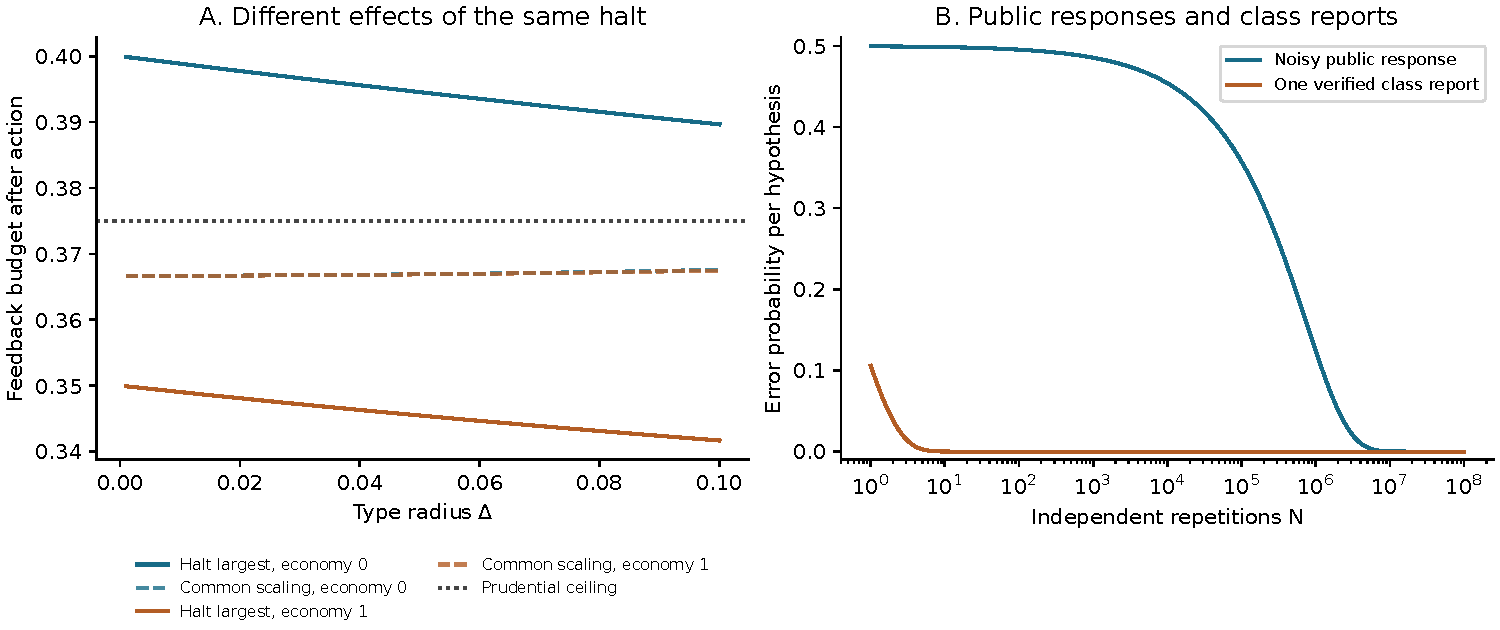
\includegraphics[width=.87\linewidth]{fig_intervention_revision.pdf}
  \caption{Intervention choice and the information value of class reports. Panel~A uses the two-class construction of Supplement Section~\ref{S-app:revisiondecision} ($a = 0.3$, $\kappa = 0.5$, $W = 0.2$, $r_c = 0.5$): a ceiling of $0.375$ separates the post-halt budgets while uniform scaling satisfies it in both economies. Panel~B fixes $\Delta = 0.05$ and compares exact likelihood-ratio error probabilities across $N$ independent repetitions (30 impulse-response coordinates vs.\ one verified class report, both with Gaussian measurement standard deviation $0.01$): achieving $5\%$ error requires roughly $2.03 \times 10^6$ public-response repetitions versus $2$ class reports (in Panel~A, the two uniform-scaling curves coincide to $O(\Delta^3)$; Panel~B is an illustrative reset benchmark rather than a live market policy).}
  \label{fig:intervention}
\end{figure}

\subsection{Minimax optimality of uniform policies}

Let class $d \in \{1, \dots, K\}$ contribute $u_d = \kappa q_d \ge 0$ to the feedback budget, with total feedback $U = \sum_{d=1}^K u_d \ge 0$ (if contrarian dealers have $u_D < 0$ as in Table~\ref{tab:taiwan}, halting an unverified label can target them and raise $S$ by $|u_D|$; Supplement Section~\ref{S-sec:mixed_sign}). A supervisory policy scales the class carrying label $c$ by $\theta_c \in [0, 1]$ at implementation cost $C(\theta)$. If $\pi$ is the unknown permutation assigning labels to underlying classes (a labeling), the post-policy budget is $S'_\pi = a + \sum_{c=1}^K \theta_c u_{\pi(c)}$ and the prudential loss is $\ell(S'_\pi)$.

\begin{theorem}[Without tags, uniform policies are minimax]\label{n:minimax}
Let $\ell:\mathbb{R}\to\mathbb{R}$ be convex and $C$ continuous, convex and permutation-invariant on $[0,1]^K$.
\begin{enumerate}
  \item[(i)] \emph{Weak dominance.} For every policy $\theta \in [0, 1]^K$, the uniform policy $\bar{\theta}\mathbf{1}$ with $\bar{\theta} = K^{-1}\sum_{c=1}^K \theta_c$ yields budget $a + \bar{\theta} U$ independent of $\pi$ and satisfies
  \[
    \ell(a + \bar{\theta} U) + C(\bar{\theta}\mathbf{1})
    \le \frac{1}{K!} \sum_{\pi} \ell(S'_\pi) + C(\theta)
    \le \max_{\pi} \ell(S'_\pi) + C(\theta).
  \]
  Labels do not enter prices (Theorem~\ref{n:suff}), so no record distinguishes labelings; the uniform policy does at least as well as $\theta$ against the worst labeling (it is minimax) and on average over labelings (it is Bayes under an exchangeable prior).
  \item[(ii)] \emph{Uniqueness.} If, in addition, $C$ is strictly convex on $[0, 1]^K$---or if $U \neq 0$, the class contributions $u_d$ are distinct, and $\ell$ is strictly convex on $[a + \sum_d \min(0, u_d),\, a + \sum_d \max(0, u_d)]$---then $\bar{\theta}\mathbf{1}$ strictly dominates every non-uniform policy $\theta \neq \bar{\theta}\mathbf{1}$, and the minimax problem admits a unique solution $\bar{\theta}^*\mathbf{1}$ (heterogeneous elastic exit is analyzed in Supplement Section~\ref{S-sec:elastic_exit}).
\end{enumerate}
\end{theorem}



The proof (Supplement Section~\ref{S-app:proofs}; formalized in Supplement Table~\ref{S-tab:newlean}) specializes the finite-group Hunt--Stein theorem (Lehmann and Romano, 2005, Chapter~8). Integrating the permutation-average inequality over the common price law extends minimax dominance to price-contingent policy rules. Halting a single unverified label guarantees a budget reduction of only the smallest class contribution, and with verified partial tags, policies uniform within each tagged group are minimax, the value of tags being the gain from tailoring intensities across groups (Supplement Corollary~\ref{S-cor:robustuniform} and Theorem~\ref{S-n:minimaxtags}).

\subsection{Class-tagged disclosure, relabeling, and the surveillance paradox}

\begin{theorem}[Statistical value of class-tagged disclosure]\label{n:disc}
Suppose that in each reset experiment of Theorem~\ref{n:cost}, each trader class's order flow is also observed at the first two response dates with independent Gaussian noise. Over any compact, uniformly stable separated family containing the hard pair and an open neighborhood of rescaled nodes and positive weights, recovering weights to a fixed accuracy below half the pair's weight gap requires $O(1)$ tagged experiments independent of $\Delta\eta$, whereas recovering memory rates to accuracy $c_0\Delta\eta$ (for sufficiently small fixed $c_0>0$) requires order $(\Delta\eta)^{-2}$ tagged experiments at fixed confidence.
\end{theorem}

As shown in Supplement Theorem~\ref{S-thm:partial}, tagging $m$ of $K$ groups lowers the composition exponent by $4$ per tag (to $4(K-m)-2$), so tagging all but one class removes the spacing penalty for weights entirely.

Crucially, however, disclosure regimes operate on strategic traders. Before solving the strategic relabeling and surveillance-crowding games, the next lemma relates their reduced-form payoffs to the inventory equilibrium of Section~\ref{sec:equilibrium} and to the steady-state Kalman trading desk of Section~\ref{sec:model}. Its welfare weight $\lambda_{\mathrm{ext}}$ is a parameter of the supervisor's criterion, not an equilibrium object, so the lemma motivates the payoffs rather than deriving them.

\begin{lemma}[Payoff foundations for disclosure and crowding]\label{lem:micro}
\begin{enumerate}
  \item[(i)] \emph{Welfare weights from equilibrium impact.} In the small-feedback equilibrium of Theorem~\ref{n:thm_inventory}(iv), each unit of aggregate feedback intensity $S_M(1) = \sum_j q_j$ raises equilibrium impact $\kappa$ by $\kappa_-^2(\bar{a} + 2A\kappa_-\sigma_\xi^2)/\sqrt{\Lambda_0} > 0$. Suppose the supervisor values a unit of feedback intensity, through the rise in impact and inventory risk it causes, at $\lambda_{\mathrm{ext}} > 0$, a parameter of its welfare criterion rather than an equilibrium object. If class $j \in \{\mathcal{H}, \mathcal{B}\}$ earns private value $b_j > 0$ per retained unit and adds $\phi_j$ to the feedback intensity, then the first-order net social value of a retained unit is $n_j = b_j - \lambda_{\mathrm{ext}} \phi_j$, yielding $n_{\mathcal{H}} < 0 < n_{\mathcal{B}}$ whenever $b_{\mathcal{H}} < \lambda_{\mathrm{ext}}\phi_{\mathcal{H}}$ and $b_{\mathcal{B}} > \lambda_{\mathrm{ext}}\phi_{\mathcal{B}}$.
  \item[(ii)] \emph{Quadratic strategy-distortion cost from Kalman filtering.} Consider a trading desk tracking a latent random-walk trend $v_{t+1} = v_t + \zeta_{t+1}$ ($\Var(\zeta) = \sigma_\zeta^2 > 0$) from noisy signals $v_t + \nu_t$ ($\Var(\nu) = \sigma_\nu^2 > 0$) with exponential memory rate $r \in (0, 1)$, using the plug-in trade $u_t=\hat v_t/(\kappa+\lambda)$ for a fixed $\kappa+\lambda>0$. Assume independent centered innovations and square-integrable initial levels, and evaluate the loss at stationary filtering error. Its stationary forecast-error variance is
  \[
    P(r) = \frac{\sigma_\zeta^2 + (1 - r)^2 \sigma_\nu^2}{1 - r^2}
         = \frac{\sigma_\zeta^2}{1 - r^2} + \frac{2\sigma_\nu^2}{1 + r} - \sigma_\nu^2,
  \]
  which is strictly convex on $(0, 1)$ with a unique minimizer $r_0 \in (0, 1)$ and $P''(r_0) > 0$. At fixed impact, deviating from $r_0$ to $r$ incurs the stationary-error profit loss
  \[
    \Pi(r_0) - \Pi(r) = \frac{P(r) - P(r_0)}{2(\kappa + \lambda)}
    = k (r - r_0)^2 + O\!\left(|r - r_0|^3\right),
    \qquad k = \frac{P''(r_0)}{4(\kappa + \lambda)} > 0.
  \]
  The expansion holds at fixed impact. It leaves open the optimal memory and local distortion cost when the desk internalizes its effect on dealer impact.
\end{enumerate}
\end{lemma}

Class tags attached to accounts prevent a trader from hiding merely by tweaking its algorithm, but a restricted trader can still route orders through accounts carrying an unrestricted label.

\begin{proposition}[Disclosure when labels can be gamed]\label{n:relabel}
Fix one supervisory cycle. A share $\chi \in (0, 1)$ of feedback activity belongs to a harmful class $\mathcal{H}$ and $1 - \chi$ to a benign class $\mathcal{B}$. Each retained unit has net social value $n_{\mathcal{H}} < 0 < n_{\mathcal{B}}$, and $\mathcal{H}$ traders earn private gain $b_{\mathcal{H}} > 0$ per retained unit. Without disclosure, the supervisor chooses a uniform retention $\theta \in [0, 1]$. With class tags, the supervisor sets retention $\theta_{\mathcal{H}}$ for label $\mathcal{H}$ and $\theta_{\mathcal{B}} \ge \theta_{\mathcal{H}}$ for label $\mathcal{B}$, and $\mathcal{H}$ traders may route a share $z \in [0, 1]$ of their activity through $\mathcal{B}$ accounts at resource cost $\gamma z^2 / 2$ per unit ($\gamma > 0$). An owner-linked audit trail prevents relabeling ($z \equiv 0$). Write $\alpha_{\mathcal{H}} = -n_{\mathcal{H}} > 0$, $m = \chi n_{\mathcal{H}} + (1 - \chi) n_{\mathcal{B}}$, $s_{\mathcal{B}} = (1 - \chi) n_{\mathcal{B}}$, and $g = \gamma / \{b_{\mathcal{H}}(2\alpha_{\mathcal{H}} + b_{\mathcal{H}})\}$.
\begin{enumerate}
  \item[(i)] \emph{Optimal hiding.} $\mathcal{H}$ traders route $z^* = \min\{1,\, b_{\mathcal{H}}(\theta_{\mathcal{B}} - \theta_{\mathcal{H}})/\gamma\}$ through $\mathcal{B}$ labels.
  \item[(ii)] \emph{Optimal policy and tag value.} Welfare is $\max\{0, m\}$ without disclosure and $s_{\mathcal{B}}$ under an audit trail (before fixed costs). Under class tags, let $V_C(\gamma)$ denote the welfare gain over the uniform cut:
  \begin{itemize}
    \item If $m \ge 0$: one optimum sets $\theta_{\mathcal{B}} = 1$, label gap $\theta_{\mathcal{B}} - \theta_{\mathcal{H}} = \min\{1, \alpha_{\mathcal{H}} g\}$, and $V_C = \chi \alpha_{\mathcal{H}}^2 g / 2$ when $\alpha_{\mathcal{H}} g \le 1$, else $V_C = \chi \alpha_{\mathcal{H}} - \chi / (2g)$.
    \item If $m < 0$: $\theta_{\mathcal{H}} = 0$, $\theta_{\mathcal{B}} = \min\{1, s_{\mathcal{B}} g / \chi\}$, and $V_C = s_{\mathcal{B}}^2 g / (2\chi)$ when $s_{\mathcal{B}} g \le \chi$, else $V_C = s_{\mathcal{B}} - \chi / (2g)$.
  \end{itemize}
  In every case, the equilibrium hiding share lies strictly in $(0, 1)$, and at interior optima it is independent of $\gamma$: $z^* = \alpha_{\mathcal{H}}/(2\alpha_{\mathcal{H}} + b_{\mathcal{H}})$ when $m \ge 0$ and $z^* = s_{\mathcal{B}}/\{\chi(2\alpha_{\mathcal{H}} + b_{\mathcal{H}})\}$ when $m < 0$.
  \item[(iii)] \emph{Audit trail versus class tags.} $V_C(\gamma)$ is continuous and strictly increasing in $\gamma$, with $V_C(\gamma) \to 0$ as $\gamma \to 0$, $V_C(\gamma) \to V_A \equiv s_{\mathcal{B}} - \max\{0, m\}$ as $\gamma \to \infty$, and $V_C(\gamma) < V_A$ for all $\gamma > 0$. Given fixed costs $F_C\le F_A$, an owner-linked trail strictly dominates if $F_A-F_C<V_A-V_C(\gamma)$. A unique finite positive cutoff applies for $0<F_A-F_C<V_A$. At zero incremental cost the trail strictly dominates for all finite $\gamma>0$; for $F_A-F_C\ge V_A$ it never strictly dominates.
\end{enumerate}
\end{proposition}

The proof (Supplement Section~\ref{S-app:proofs}) yields three economic consequences. First, cheap relabeling restores observational equivalence in equilibrium: as $\gamma \to 0$, class tags become worthless. Second, a harmful label is left partly open in the interior case with positive net value of uniform retention. At a boundary it may be closed. When $m<0$ the supervisor can restrict the benign label because it serves as the hiding channel. Third, an owner-linked audit trail preserves its full value $V_A$ only when beneficial ownership is not severed by synthetic offshore total-return swaps ($\gamma_{\mathrm{TRS}}$) or multi-desk netting inside a single legal entity. In practice, the Consolidated Audit Trail shows both the governance costs $F_A$ and what owner-level linkage needs. In 2025 the SEC exempted the reporting of names, addresses and years of birth of U.S.\ natural persons, and CAT LLC proposed removing all personally identifying information; regulators would still be able to tell whether trading in several accounts belongs to the same customer, which is the linkage the model needs, without knowing who the customer is (Securities and Exchange Commission, 2025; FINRA, 2025). The SEC's 2023 funding order was vacated in \emph{American Securities Association v.\ SEC}, No.~23-13396 (11th Cir.\ July 25, 2025) (Supplement Section~\ref{S-app:relabel}), while firm-assigned labels remain gameable (Frankel and Kartik, 2022; Perez-Richet and Skreta, 2022). While Proposition~\ref{n:relabel} adopts linear per-unit values $(n_{\mathcal{H}}, n_{\mathcal{B}})$ for closed-form transparency, Supplement Theorem~\ref{S-thm:relabelgeneral} extends the limits to Lipschitz social welfare and private payoffs with slopes bounded above and bounded away from zero, under the stated routing-cost conditions. The cheap-routing collapse requires all labels to be reachable. This covers quadratic aggregate-feedback stability externalities $U(e) = \sum_j \chi_j b_j e_j - \frac{\lambda}{2}(\sum_j \chi_j w_j e_j)^2$ directly linked to the feedback budget of Section~\ref{sec:equilibrium}.

Even without account relabeling, an untagged algorithm that anticipates targeting can disguise itself by shifting its trading rule toward its neighbor's, at a cost to its own strategy. The next result characterizes what the supervisor learns when the algorithm best-responds to a fixed test.

\begin{theorem}[The surveillance paradox]\label{n:paradox}
Consider an untagged group that chooses the distance $\delta \in [0, \delta_0]$ between its memory rate and its neighbor's at strategy-distortion cost $k(\delta_0 - \delta)^2$, holding all other groups fixed ($\delta_0, k > 0$). From $N$ observations, the supervisor tests at level $\alpha \in (0, 1/2)$ the composite null that the two groups merge into a single group of unknown memory and weight; rejection triggers an inquiry costing the group $L > 0$. Suppose the Kullback--Leibler divergence from the economy at distance $\delta$ to the closest null economy satisfies $J = c N \delta^n$ on $[0, \delta_0]$ with $c > 0$ and $n > 2$, and the test's power depends on the alternative only through $J$, through a continuous function $P_{\mathrm{d}}(J) \ge \alpha$ with $P_{\mathrm{d}}(0) = \alpha$. Every level-$\alpha$ test satisfies the Pinsker envelope $P_{\mathrm{d}}(J) - \alpha \le \sqrt{J/2}$, which part~(i) uses. Let $\delta^*$ minimize $k(\delta_0 - \delta)^2 + L P_{\mathrm{d}}(c N \delta^n)$ and set $J^* = c N (\delta^*)^n$.
\begin{enumerate}
  \item[(i)] \emph{Hiding is never complete.} Against every such test, $\delta^* > 0$, and $(\delta^*)^{n-2} \ge 2 k^2 \delta_0^2 / (2^n L^2 c N)$ whenever $\delta^* \le \delta_0 / 3$.
  \item[(ii)] \emph{A good test forces crowding.} If the test's power satisfies $P_{\mathrm{d}}(J) - \alpha \ge \beta \min\{\sqrt{J}, \sqrt{\bar{J}}\}$ and the stakes are high ($L \beta \sqrt{\bar{J}} > k \delta_0^2$), then for every $N$,
  \[
    (\delta^*)^{n-2} \le \frac{4 k^2 \delta_0^2}{L^2 \beta^2 c N}.
  \]
  \item[(iii)] \emph{More data, less information.} Against such a test, for all large $N$, $\delta^* \asymp N^{-1/(n-2)}$ and the supervisor's information obeys $J^* \asymp N^{-2/(n-2)} \to 0$ ($N^{-1}$ in the benchmark $n=4$): detection probability tends to $\alpha$, and distortion cost $k(\delta_0 - \delta^*)^2$ tends to $k \delta_0^2$.
  \item[(iv)] \emph{Tag-based inquiry.} Under a verified class tag whose inquiry probability is independent of $\delta$, the unique optimum is $\delta^* = \delta_0$, and the group's rule is estimable from tagged flow (Theorem~\ref{n:disc}).
\end{enumerate}
\end{theorem}

The exponent $n$ reflects the composite null: because prices do not reveal the neighbor's memory, a single merged group matching total weight $W = w_1 + w_2 \neq 0$ and mean memory cancels linear differences and leaves an $O(\delta^2)$ kernel gap and $O(\delta^4)$ divergence ($n = 4$; fitted spectral slope $4.1$ in Supplement Section~\ref{S-app:paradox}, vs.\ $n = 8$ for three-group clusters). By contrast, opposite-sign pairs ($w_1 = -w_2$) or a known simple null yield $n = 2$, permitting complete hiding once $N$ is large. In a Gaussian shift experiment along a known normal direction, a one-sided test satisfies~(ii) with $\beta = \sqrt{2}\phi(z_\alpha)$ and $\bar{J} = z_\alpha^2 / 2$ (Appendix~\ref{app:proofs}), whereas an unknown sign requires a composite-null GLRT ($P_{\mathrm{d}}(J) - \alpha = c_2 J + O(J^2)$) that slows crowding to $\delta_N^* \asymp N^{-1/(n-1)}$.

Economically, untagged surveillance provokes crowding that more than offsets additional observations, imposing a permanent strategy-distortion loss $k(\delta_0 - \delta)^2$ (microfounded by Kalman filtering in Lemma~\ref{lem:micro}(ii)). If the conduct at $\delta_0$ is itself harmful, this crowding acts as deterrence; what fails is supervisory learning rather than necessarily welfare---mirroring how policy intervention degrades market signals (Bond et al., 2010; Bond and Goldstein, 2015; Frankel and Kartik, 2019). Without an inquiry cost $L > 0$, detection has no behavioral bite (Theorem~\ref{n:minimax}). When multiple untagged groups position simultaneously, Supplement Proposition~\ref{S-prop:hidegame}(iv) bounds asymptotic detection across any pure-strategy Nash equilibrium with bounded neighbor distances, while memory-independent tag inquiries eliminate crowding altogether. If the supervisor also chooses how hard to monitor, crowding makes committed monitoring unprofitable for large records under high stakes, and equilibrium auditing must be randomized (Supplement Proposition~\ref{S-prop:endogenous_supervisor}).

\textbf{What a longer price record buys.} Theorem~\ref{n:paradox} is about detection; a supervisor deciding what to record needs the value of what it learns. Compare the price record with a record that links accounts to their owners.

\begin{theorem}[More data does not substitute for records]\label{n:recordvalue}
Consider one supervisory cycle with two equally likely states: in state $1$ the untagged group of Theorem~\ref{n:paradox} is present at distance $\delta$ from its neighbor, and in state $0$ the record comes from the closest merged economy. A policy $\theta$ in a compact set $\Theta$ earns welfare $W(\theta, \omega)$, continuous in $\theta$. Let $W_\varnothing = \max_\theta \tfrac12\{W(\theta, 0) + W(\theta, 1)\}$ be the best welfare without information, and $V^* = \tfrac12\{\max_\theta W(\theta, 0) + \max_\theta W(\theta, 1)\} - W_\varnothing \ge 0$ the value of knowing the state, which an owner-linked record supplies.
\begin{enumerate}
  \item[(i)] \emph{Value of a record.} Every policy chosen from a record whose laws in the two states are $P_0$ and $P_1$ gains at most $\TV(P_0, P_1)\, V^* \le V^* \sqrt{\KL(P_1 \| P_0)/2}$ over $W_\varnothing$.
  \item[(ii)] \emph{The price record under crowding.} Suppose the supervisor targets through a test as in Theorem~\ref{n:paradox}(ii), a rejection costs the group $L$, and stakes are high. Let $V_P(N)$ be the gain of any policy based on $N$ price observations when the group crowds optimally against the test. In the benchmark $n = 4$, for every $N$,
  \[
    V_P(N) \le \frac{2\sqrt{2}\, k^2 \delta_0^2}{L^2 \beta^2 \sqrt{cN}}\, V^*,
  \]
  and for general $n > 2$, $V_P(N) \le V^* \{c N B_N^{n/(n-2)}/2\}^{1/2}$ with $B_N = 4k^2\delta_0^2/(L^2\beta^2 cN)$, which is of order $N^{-1/(n-2)}$. If the test is instead two-sided, with $P_{\mathrm{d}}(J) - \alpha \ge \beta_2 \min\{J, \bar J\}$ and $L\beta_2 \bar J > k\delta_0^2$, then $(\delta^*)^{n-1} \le 2k\delta_0/(L\beta_2 cN)$ and
  \[
    V_P(N) \le \frac{V^*}{\sqrt 2}\Bigl(\frac{2k\delta_0}{L\beta_2}\Bigr)^{n/(2(n-1))} (cN)^{-1/(2(n-1))},
  \]
  of order $N^{-1/6}$ at $n = 4$.
  \item[(iii)] \emph{Record choice.} If $V^* > 0$ and an owner-linked record costs $F_A < V^*$, it is strictly better than targeting from prices once
  \[
    N > \frac{8 k^4 \delta_0^4 (V^*)^2}{L^4 \beta^4 c\, (V^* - F_A)^2} \qquad (n = 4),
  \]
  and at every record length the price record's gain stays strictly below $V^*$.
\end{enumerate}
\end{theorem}

Part~(i) is the standard bound on the value of an experiment (Blackwell, 1953; Le Cam, 1964). The content is in~(ii) and~(iii). Because the group crowds as the record grows, the value of price surveillance is at most of order $N^{-1/2}$ against a one-sided test and $N^{-1/6}$ against a two-sided one, so a longer price record does not substitute for an owner-linked one, and the record length beyond which a trail of cost $F_A$ pays is explicit. The statement is about the group's best response to a fixed test, not an equilibrium with an optimizing supervisor (for that, see Supplement Proposition~\ref{S-prop:endogenous_supervisor}). Proposition~\ref{n:relabel} compares owner-linked trails with class tags at fixed costs; Theorem~\ref{n:recordvalue} adds the comparison with prices alone. In the Gaussian shift experiment with $\alpha = 0.05$, $k = 1$, $\delta_0 = 0.2$, $L = 1$ and $c = 1$ (replication archive), the bound in~(ii) holds at every $N$ from $10$ to $10^8$, and the exact total variation falls with fitted slope $-0.48$ in $\log N$ for $N \ge 10^4$ ($-0.37$ over the whole range, before the asymptotic regime sets in).


\subsection{Illustrative empirical calibration: Taiwan Stock Exchange tagged flows}\label{sec:taiwan}

To illustrate the magnitude of the identification barrier in an actual exchange dataset, we examine the decision problem in Theorems~\ref{n:cost} and~\ref{n:dual} using daily class-tagged net buying from the Taiwan Stock Exchange (TWSE) across three reported institutional classes---foreign investors, investment trusts, and dealers---over 2013--2016 ($300$ stocks, $270{,}060$ stock-days). We estimate each class's persistence $r_c$ and response $w_c$ to the prior day's price deviation, along with the market's lagged-flow impact $\kappa$ and price persistence $\sum_{j=1}^5 a_j$, using stock fixed effects and stationary date-block bootstrap confidence intervals (Table~\ref{tab:taiwan}). For each stock, $x_t$ is the event-adjusted basis $\log P_t - \hat\beta \log\mathrm{TAIEX}_t$ minus its trailing 60-day mean, with $u_{c,t}$ reacting to $x_{t-1}$ and $x_t$ loading on $U_{t-1}$ (a two-day feedback loop; Supplement Section~\ref{S-app:barrier}).\footnote{\label{fn:persist}Trailing 60-day demeaning of a random walk alone produces first-order persistence $118/121 = 0.975$, and the estimated $\sum_j \hat a_j = 0.972$ is close to that value, so the price persistence in Table~\ref{tab:taiwan} is largely a property of the filter, not evidence about how pricing errors decay. First-differencing $\Delta x_t$ and excluding price-limit days leave the class flow persistences $\hat r_c$ nearly unchanged (Figure~\ref{fig:twse_sensitivity}B; Supplement Table~\ref{S-tab:p1m_sensitivity}), but not the responses: under first differencing $\hat w_F = -1.82$ and $\hat w_D = -0.55$, so the sign of foreign feedback depends on the specification.} Market structure shapes these daily series: TWSE had reduced its periodic call-auction interval in four steps from 25 to 5 seconds between 2010 and 2014 (Twu and Wang, 2018), expanded day trading in 2014, widened daily price limits ($\pm 7\%\to\pm 10\%$, June~2015), publishes daily post-close institutional summaries permitting next-day copycatting outside Theorem~\ref{n:suff}, and shifted to continuous matching on 23~March~2020. In addition, aggregate dealers ($w_D = -0.022$) combine warrant hedging with proprietary dealer accounts (\texttt{DealerOwn}, $\hat w = +0.00295$), while unconstrained distributed lags show a day-1 reversal followed by multi-day persistence, consistent with (but not shown to be) the slicing of parent orders by TWAP/VWAP algorithms ($\hat\beta_{F,1} = -1.235$ vs.\ lags $+0.741, +0.496$; Supplement Section~\ref{S-app:barrier}).

\begin{table}[!htbp]
\centering
\caption{Estimated tagged trading rules in Taiwan, 2013--2016 (300 stocks, 270,060 stock-days; stock fixed effects with 95\% date-block bootstrap intervals, mean block 20). The rules assume that each class's feedback decays at its own flow persistence and a common impact $\kappa$ for all classes.}
\label{tab:taiwan}
\small
\begin{tabular}{@{}lccc@{}}
\toprule
Trader class & Persistence $r_c$ & Price response $w_c$ & Budget contribution $u_c = \kappa w_c / (1 - r_c)$ \\
\midrule
Foreign investors & $0.35 \; [0.31, 0.38]$ & $0.24 \; [0.21, 0.27]$ & $0.0014 \; [0.0012, 0.0016]$ \\
Investment trusts & $0.41 \; [0.39, 0.43]$ & $0.066 \; [0.057, 0.076]$ & $4.2 \times 10^{-4} \; [3.3 \times 10^{-4}, 5.3 \times 10^{-4}]$ \\
Dealers           & $0.33 \; [0.22, 0.42]$ & $-0.022 \; [-0.028, -0.017]$ & $-1.3 \times 10^{-4} \; [-1.8 \times 10^{-4}, -8.2 \times 10^{-5}]$ \\
\midrule
\multicolumn{4}{@{}p{0.97\linewidth}}{\footnotesize Lagged-flow price impact $\kappa = 0.0038 \; [0.0032, 0.0044]$; aggregate price persistence $\sum_{j=1}^5 a_j = 0.97$, about what the detrending filter alone implies.} \\
\multicolumn{4}{@{}l}{\footnotesize Within-stock $R^2$: price equation $0.95$; rules $0.14$ (Foreign), $0.18$ (Trust) and $0.10$ (Dealers).} \\
\bottomrule
\end{tabular}
\end{table}

\begin{figure}[!htbp]
  \centering
  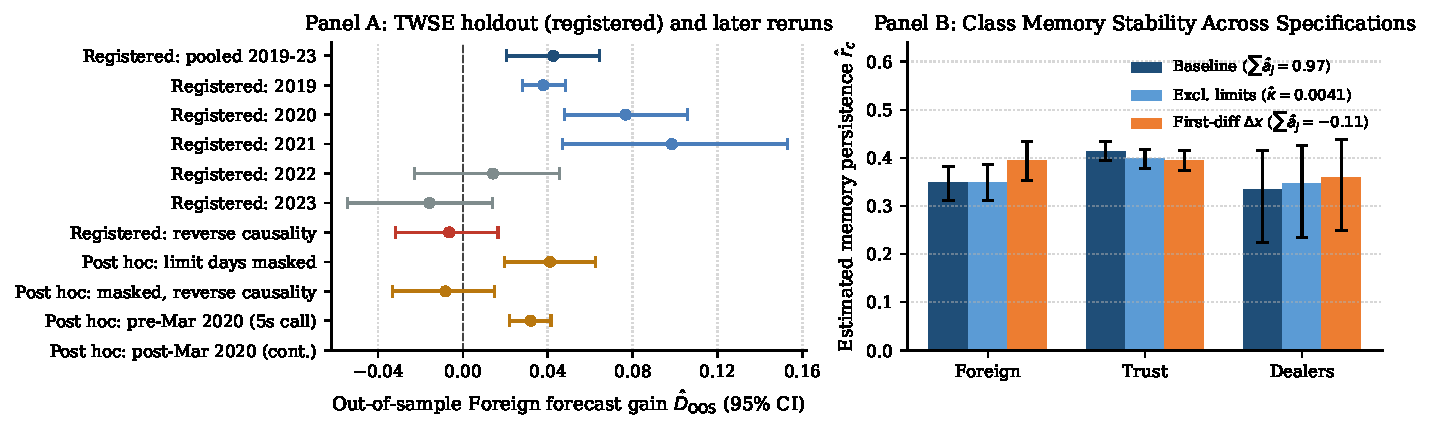
\includegraphics[width=.80\linewidth]{fig_twse_sensitivity.pdf}
  \caption{TWSE 2019--2023 out-of-sample holdout and specification sensitivity. Panel~A: foreign proportional MSE gain $\hat{D}_{\mathrm{OOS}}$ with $95\%$ block-20 intervals. Rows marked ``registered'' are the registered holdout (pooled $0.0426$, annual subsamples, pre-specified reverse-causality check $-0.0065$); rows marked ``post hoc'' were run after the holdout was opened and are not registered (limit and post-halt days masked, $0.0410$; split at the 23~March~2020 switch to continuous matching, which coincided with the COVID-19 sell-off, $0.0319$ and $0.0421$). Panel~B: estimated persistence $\hat{r}_c$ ($95\%$ CI) across Baseline, Limit-Excluded ($\hat{\kappa}=0.00409$), and First-Differenced $\Delta x_t$ ($\sum \hat{a}_j=-0.109$, $\hat{\kappa}_{\Delta x}=0.00209$).}
  \label{fig:twse_sensitivity}
\end{figure}

Granting a price-only supervisor full knowledge of the impact function $\kappa$ and the law of non-feedback order flow (so only class composition is unknown) yields three quantitative contrasts (Supplement Section~\ref{S-app:barrier}, which specifies the search). Price and tagged records are compared against separately optimized single-memory candidates with non-feedback flow held at its estimated law; the ranges below are endpoints of local searches, not certified extrema.
\begin{enumerate}
  \item \emph{Information.} Against their respective fitted single-memory alternatives, one stock-day of prices carries an estimated $1.7 \times 10^{-12}$~nats about class composition and one stock-day of tagged flows $8.0 \times 10^{-7}$~nats. Both are small in absolute terms. The whole 2013--2016 tagged panel carries $270{,}060 \times 8.0 \times 10^{-7} = 0.22$~nats, so by Pinsker's inequality any tagged-flow test of memory composition has power minus size at most $0.33$; for prices the bound is $4.8 \times 10^{-4}$. Power minus size $0.75$ ($80\%$ power at $5\%$ size) needs $1.125$~nats by the same inequality: $2.7 \times 10^9$ years of prices for one stock ($9.1 \times 10^6$ years for 300 independent stocks) at the panel's $245.5$ trading days a year, against $5{,}700$ years of tags for one stock ($19$ years for 300 stocks). Table~\ref{tab:years} uses a different conversion (the Bretagnolle--Huber bound $\ln 5/D$ at $252$ days), so the two sets of years are not comparable. In Taiwan, then, the tags identify class contributions only under the maintained restriction that feedback memory equals flow persistence; they do not identify the feedback memories themselves.
  \item \emph{Targeted halt.} With tags, halting foreign feedback lowers the feedback budget by $0.0014$ ($95\%$ CI $[0.0012, 0.0016]$). On the class the lower bounds cover (every weight nonnegative, memories in $[0, 0.99]$), the compositions the panel cannot tell apart imply contributions of foreign feedback from $0$ to $0.0018$, against a uniform cut between $0.0016$ and $0.0018$ on the same class, so prices leave foreign feedback anywhere between none and all of the total. For one stock the ranges are $[0, 0.0035]$ and $[1.3 \times 10^{-4}, 0.0046]$ and overlap. Holding each class's weight to the sign of its tagged estimate, so that the contrarian dealers can offset the others at nearby memories, gives $[0, 0.028]$, which fills the cap on each class's contribution; allowing weights of either sign gives $[-0.028, 0.028]$, attained only at negative memory rates, outside the model's $r \in (0, 1)$. Permutation relabeling alone leaves $0.0014$, $4.2 \times 10^{-4}$ and $-1.3 \times 10^{-4}$ observationally equivalent at every record length.
  \item \emph{Uniform feedback reduction.} On the nonnegative class, setting total feedback to zero lowers the budget by $0.0016$ to $0.0018$ across the price-consistent candidates.
\end{enumerate}

Four qualifications apply. First, the tagged intervals in Table~\ref{tab:taiwan} assume a common impact and that each class's feedback decays at its own flow persistence. With the class-specific impacts the price equation estimates as a diagnostic ($0.0035$, $0.012$ and $-0.0004$; Supplement Section~\ref{S-app:barrier}), the point contributions become $0.0013$ (foreign), $0.0013$ (trusts) and $1.4 \times 10^{-5}$ (dealers), so which class is largest depends on that restriction; we have not tested equal impacts. With feedback decoupled from each class's flow persistence (a free ten-day distributed lag of $x$, with second-order autoregressive non-feedback flow), foreign feedback contributes $0.0013$ ($95\%$ interval $[0.0011, 0.0015]$). Second, item~3 rests on the grant: the price-only supervisor is given the persistences $a_j$, the impact $\kappa$ and the non-feedback law, all estimated with the tagged flows; with feedback contributing $0.0017$ to a budget of $0.97$, separating the two from prices alone is the problem that Proposition~\ref{n:target} assumes away. Third, we have not recomputed the information measures and ranges under the first-differenced and limit-excluded specifications, where the responses change sign (footnote~\ref{fn:persist}). Fourth, the calendar-year conversions assume cross-stock independence (whereas the common-date bootstrap accommodates cross-stock dependence), and dealers' negative $w_D$ lies outside the positive class (though Whittle rates, Pinsker's inequality, and relabeling invariance still apply).

Two further caveats concern the data. First, daily institutional flows exhibit small lagged price impact ($\kappa = 0.0038$), contributing $0.0017$ to an overall persistence budget of $0.97$ at this daily frequency; thus Table~\ref{tab:taiwan} illustrates the \emph{relative} identification gap between uniform and targeted interventions rather than claiming that daily institutional flows destabilize Taiwanese equities. Second, the registered 2019--2023 out-of-sample holdout (spec P1T; Supplement Section~\ref{S-sec:p1t}) asks whether the price deviation improves out-of-sample forecasts of a class's own tagged flow beyond the flow's two lags; $\hat D_{\mathrm{OOS}}$ is the mean across stocks of the proportional MSE reduction. In the words fixed before the holdout was opened: ``$D = 0.0426$ $[0.0206, 0.0643]$, $p = 0.000$, meets the registered supportive criterion. The pre-specified reverse-causality check gives $D = -0.0065$ $[-0.0316, 0.0165]$, which does not meet it. The registered verdict is `supportive'. Read with its pre-specified diagnostic, the test does not provide evidence of feedback beyond prices revealing past flow.'' The reported $p = 0.000$ is rounded: no centred bootstrap resample out of $9{,}999$ reached $D$, so $p < 10^{-4}$. The check replaces $x_t$ by its residual from a fit-period regression on $x_{t-1}$ and lagged reported flows. Supplement Table~\ref{S-tab:p1t_all} reports every registered outcome. Among them, the price deviation worsens out-of-sample forecasts of investment-trust flow ($D = -0.0493$, $[-0.0950, -0.0114]$) and does not improve those of dealers' own flow ($D = -0.0025$), so the trust response in Table~\ref{tab:taiwan} has no out-of-sample support; and the per-stock tagged instrumental-variable estimates of the foreign flow memory lie outside $(-1, 1)$ for 286 of 293 stocks (median $1.32$ in the fit period), so they do not measure memory stock by stock. Two later analyses were not registered: masking price-limit and post-halt days gives $0.0410$ $[0.0197, 0.0623]$ with reverse-causality check $-0.0083$ $[-0.0332, 0.0150]$, and splitting at the 23~March~2020 switch to continuous matching, which coincided with the COVID-19 sell-off, gives $0.0319$ before and $0.0421$ after. In the words fixed before the holdout was opened: ``We do not claim that tagged flow in Taiwan responds to price deviations. The registered test is supportive, but its pre-specified diagnostic attributes the gain to reverse causality.'' Positive feedback in foreign flows is documented across markets (Froot et al., 2001; Griffin et al., 2004; Richards, 2005), while Wu and Wang (2020) measure turnover rather than signed trader-type feedback. Accordingly, these figures serve as an illustrative calibration of the relative identification gap between uniform and targeted cuts rather than a causal test of daily feedback destabilization; evaluating a high-feedback venue would require separate evidence on whether shares $\kappa\sum_i q_i$ are economically larger (as in the Section~\ref{sec:cost} and Supplement Section~\ref{S-app:revisiondecision} parameterizations underlying Figures~\ref{fig:near-instability} and~\ref{fig:intervention}), where the same $(\Delta\eta)^{-(4K-2)}$ barrier carries direct prudential weight.

\section{Scope and Conclusion}\label{sec:conclusion}

Prices tell a supervisor how much feedback a market carries, not who carries it. Under mechanical price impact and in an inventory-dealer equilibrium, the pricing-error response identifies the aggregate kernel under the observation conditions of Sections~\ref{sec:equilibrium} and~\ref{sec:cost}, while separating closely spaced trader classes costs of order $\Delta^{-(4K-2)}$ observations, and that cost does not fall as the market nears instability.

Three policy conclusions follow. First, a market-wide cut is the natural default when targeting cannot be verified. Without tags it is minimax over labelings. With persistence, impact and a memory bound given, its effect is learned from one passive pricing-error record at a cost that does not depend on how close the traders' memories are (Theorems~\ref{n:separation} and~\ref{n:passiveupper}). In the dealer equilibrium, on the principal branch, a cut still lowers the budget and its effect is learned without the spacing penalty, though more slowly (Theorem~\ref{n:eqcut}); on a lower branch a uniform cut raises the budget, so the default needs the market to sit on the principal equilibrium. Smooth quadratic charges can likewise be evaluated from pricing errors alone, unlike proportional taxes and binding caps (Supplement Proposition~\ref{S-thm:instruments}). Second, a class-specific restriction needs attribution, and there are two ways to obtain it: verified flow tags remove the spacing penalty for weights, and a pilot of the restriction reveals its effect from prices after the fact (Theorem~\ref{n:pilot}). Third, tags are fragile when traders respond to them. Routing orders across labels erodes them, and untagged surveillance invites crowding that no longer record undoes (Theorems~\ref{n:paradox} and~\ref{n:recordvalue}). Records linked to beneficial owners, such as the cross-venue customer linkage in consolidated audit trails, can support targeted supervision to the extent that those links hold.

The results have limits. The explicit identification and upper-bound theorems use linear causal rules with exponential or smooth memory; drifting populations, hard position limits, breach cascades, and saturating or learning algorithms are analyzed in the companion working papers (Niroula et al., 2026c, 2026d). The passive bounds require Gaussian (or quadratically regular) innovations and exclude bounded-support laws. Theorem~\ref{n:paradox} fixes the test; when the supervisor also chooses how hard to monitor, high stakes give either Stackelberg collapse or mixed-strategy auditing (Supplement Proposition~\ref{S-prop:endogenous_supervisor}), and repeated reputation is left out. The Taiwan illustration holds persistence and impact fixed, its persistence is largely produced by detrending, and it relies on asymptotic rate proxies, so pure causal feedback and cross-stock independence remain open, and discrete time abstracts from continuous-book cancellations and sub-millisecond races (Supplement Sections~\ref{S-sec:scope} and~\ref{S-sec:natural_experiments}, Proposition~\ref{S-prop:natural_exp}). A direct causal test of the separation would evaluate an exogenous, externally documented class-specific restriction against pre-specified predictions; Theorem~\ref{n:pilot} states the prediction such a test would check.

\section*{Declarations}

\textbf{Author contributions (CRediT).} Pratik Niroula: conceptualization, methodology, formal analysis, software (numerical scripts, empirical executors and Lean~4 files, written with the AI assistance described below), investigation, data curation, writing (original draft). Prashant Niroula: validation (proofs, Lean~4 formalizations, and empirical calculations), writing (review and editing). Sujan Khatiwada: validation (proofs, Lean~4 formalizations, and empirical calculations), writing (review and editing). All authors approved the final manuscript.

\textbf{Related manuscripts.} An earlier working paper of the same authors (Niroula et al., 2026a, dated 5 November 2026) studied the same model; this article supersedes it. Niroula et al.\ (2026b), with a different author list (P.~Niroula, S.~Alkhushayni, Y.~Chen, M.~Bhavsar and P.~Niroula), studies transient amplification and pre-trade guards; it is cited once, for a fact no result here uses. The companion note (Niroula et al., 2026c) and the full working paper (Niroula et al., 2026d) collect results this article does not use. All four are unpublished working papers in the repository cited below, and none is under consideration at a journal or conference.\par\medskip

\textbf{Funding and competing interests.} This research received no external funding. The authors declare no competing interests.

\textbf{Data and code availability.} The empirical data are public. Taiwan Stock Exchange daily reports T86, MI\_INDEX, FMTQIK and TWT49U (\url{https://www.twse.com.tw}) were downloaded on 7--8 November 2026; the download manifest with the SHA-256 of every response is in the replication archive (Supplement Section~\ref{S-sec:p1t}). Supplement Section~\ref{S-sec:scope} also cites tests on Binance public futures data (\url{https://data.binance.vision}) and CFTC Commitments of Traders reports (\url{https://www.cftc.gov}); their specifications and results files are in the archive. Empirical protocols, executors, results files, numerical checks and Lean~4 files are at \url{https://github.com/Pratikn03/Fianince}.

\textbf{Declaration of generative AI and AI-assisted technologies in the research and writing process.} The authors used Claude (Anthropic; Claude Opus 5.5 and Claude Fable 5.2, the versions recorded in the repository's commit history), ChatGPT/Codex (OpenAI) and Gemini (Google; versions not recorded). In the research process these tools wrote, at the authors' direction, the numerical verification scripts, the empirical executors and notebooks, and the Lean~4 files, and checked literature (Supplement Section~\ref{S-app:verification}); the authors ran every empirical notebook, and each registered test was run once by the first author. In writing, they were used for drafting and language editing. After using these tools, the authors reviewed, verified and edited all mathematical proofs, calculations and prose through 27 November 2026 and take full responsibility for the content of the publication. The revision of 28 November 2026, which responds to AI-generated referee reports, is being checked by the authors; until they finish, its new statements have been checked numerically (replication archive) but not yet by the authors. Lean~4 checks certify the formal statements listed in Supplement Table~\ref{S-tab:claims}, not their correspondence with the prose, empirical validity, or novelty.

\appendix
\small\linespread{0.94}\selectfont
\setlength{\parskip}{1.5pt plus 0.5pt minus 0.5pt}
\setlength{\abovedisplayskip}{2pt plus 1pt minus 1pt}
\setlength{\belowdisplayskip}{2pt plus 1pt minus 1pt}
\setlength{\abovedisplayshortskip}{1pt plus 1pt}
\setlength{\belowdisplayshortskip}{1pt plus 1pt}
\section{Proofs of Main Economic Results}\label{app:proofs}

\noindent This appendix proves the headline results. The proofs of the other main-text results, extended derivations, and the exact mapping between deterministic proof steps and Lean~4 formalizations appear in the Online Supplement (Sections~\ref{S-app:proofs} and~\ref{S-app:verification} and Table~\ref{S-tab:newlean}).

\begin{proof}[Proof of Theorem~\ref{n:suff}]
We argue by strong induction on $t \le T$ for any fixed strategy profile $(X, P)$ and realization $(v, z)$. Suppose prices and total order flows coincide across the two economies for all dates $j < t$. Then: (1) public signals $s_j = \mathcal{S}_j(p_0, \dots, p_j)$ coincide for all $j < t$; (2) aggregate feedback flow $f_t = \sum_{m < t} k_m s_{t-1-m}$ coincides because $k_m = k'_m$ for $m < T$; (3) the insider's order $X_t(v, \mathcal{H}_{t-1})$ coincides by causality; and (4) total order flow $Y_t = X_t + z_t + f_t$ and the dealer's price $P_t(\mathcal{H}_{t-1}, Y_t)$ coincide by causality. Hence price and flow paths, realized insider profit $\sum_{t \le T}(v - p_t) X_t$, and dealer inventory $-\sum_{t \le T} Y_t$ coincide pathwise. Because strategy sets and expected payoffs over $(v, z)$ are identical, best-response correspondences and equilibria coincide under any solution concept defined from public histories and payoffs. For any finite linear population with individual kernels $\kappa^{(j)}$, $f_t = \sum_j \sum_{m < t} \kappa_m^{(j)} s_{t-1-m} = \sum_{m < t} k_m s_{t-1-m}$ with $k = \sum_j \kappa^{(j)}$, so the identical induction applies.
\end{proof}

\begin{proof}[Proof of Theorem~\ref{thm:what-id}]
With $x_{-1} = 0$ and zero initial group states, each group's state obeys $y_{i,t} = \sum_{s \le t} \eta_i r_i^{t-s} x_s$. Aggregating over groups gives total feedback flow $\sum_i q_i y_{i,t} = \sum_{s \le t} k_{t-s} x_s$. By induction on $t$, pricing errors $x_t$ under probe sequence $v_t$ are determined uniquely by $(a, \kappa)$ and the feedback kernel $k_m = \int r^m \, dM(r)$, hence by the merged measure $M$. Conversely, matching price responses to all probe sequences requires matching impulse responses $h_j$ for all $j \ge 0$, uniquely identifying the closed-loop transfer function $H(z)$ and the feedback transfer $G(z) = \sum_{m \ge 0} k_m z^{-m} = \sum_i w_i z / (z - r_i)$. Partial fraction decomposition of $G(z)/z = S_M(z)$ uniquely identifies its poles $r_i \in (0,1)$ and nonzero merged weights $w_i$, uniquely recovering $M = \sum_i w_i \delta_{r_i}$ (Supplement Section~\ref{S-sec:suff} and Theorem~\ref{S-thm:merged}).
\end{proof}




\begin{proof}[Proof of Theorem~\ref{n:passiveupper}]
Because $y_{i,t-1} = \eta_i \sum_{j \ge 0} r_i^j x_{t-1-j}$, equation~\eqref{eq:baseline} with $v_t \equiv 0$ reads $x_t - a x_{t-1} = \sum_{j \ge 0} \theta_j x_{t-1-j} + \varepsilon_t$ with $\theta_j = \kappa k_j \ge 0$. Let $A(z) = 1 - a z - \sum_{j \ge 0} \theta_j z^{j+1}$. On $|z| \le 1$, $|A(z) - 1| \le a + \sum_j \theta_j = S \le 1 - m$, so $A$ has no zero in the closed disc, the record is causal in the news, and $m \le |A(e^{i\omega})| \le 2$. The spectral density $f = \sigma^2 / (2\pi |A(e^{-i\omega})|^2)$ lies in $[\sigma^2/(8\pi), \sigma^2/(2\pi m^2)]$, so the covariance matrix $\Gamma$ of $X_t = (x_{t-1}, \dots, x_{t-L})$ has eigenvalues in $[\sigma^2/4, \sigma^2/m^2]$, $\gamma(0) \le \sigma^2/m^2$, and by Parseval $\sum_u \gamma(u)^2 = 2\pi \int f^2 \le \sigma^4/m^4$.

Write $x_t - a x_{t-1} = X_t^\top \theta_{0:L-1} + \varrho_t + \varepsilon_t$ with $\varrho_t = \sum_{j \ge L} \theta_j x_{t-1-j}$, so that $\hat\theta - \theta_{0:L-1} = \hat\Gamma^{-1} T^{-1} \sum_t X_t (\varrho_t + \varepsilon_t)$ with $\hat\Gamma = T^{-1} \sum_t X_t X_t^\top$. (a) For a stationary Gaussian record each entry of $\hat\Gamma - \Gamma$ has variance at most $2 T^{-1} \sum_u \gamma(u)^2$, so $E\|\hat\Gamma - \Gamma\|_F^2 \le 2 L^2 \sigma^4 / (m^4 T)$; by Chebyshev's inequality $\|\hat\Gamma - \Gamma\|_{\mathrm{op}} \le \sigma^2/8$, hence $\|\hat\Gamma^{-1}\|_{\mathrm{op}} \le 8/\sigma^2$, with probability at least $1 - 128 L^2/(m^4 T) \ge 1 - \beta$. (b) $\varepsilon_t$ is independent of $(X_s, \varepsilon_s, X_t)$ for $s < t$, so $E\|T^{-1} \sum_t X_t \varepsilon_t\|^2 = L \gamma(0) \sigma^2 / T$, and this norm is at most $\sigma^2 \sqrt{L/(m^2 T \beta)}$ with probability at least $1 - \beta$. (c) $\operatorname{Var} \varrho_t \le \rho_L^2 \gamma(0)$ with $\rho_L \ge \sum_{j \ge L} \theta_j$, so $E\|T^{-1} \sum_t X_t \varrho_t\| \le \sqrt{L}\, \gamma(0) \rho_L$, and this norm is at most $\sqrt{L}\, \sigma^2 \rho_L / (m^2 \beta)$ with probability at least $1 - \beta$. On the intersection, $\|\hat\theta - \theta_{0:L-1}\|_2 \le 8\sqrt{L}\{(m\sqrt{T\beta})^{-1} + \rho_L/(m^2\beta)\}$, the displayed bound; and $|\hat S - S| = |\sum_{j < L} (\hat\theta_j - \theta_j) - \sum_{j \ge L} \theta_j| \le \sqrt{L}\, \|\hat\theta - \theta_{0:L-1}\|_2 + \rho_L$.

\emph{(i)} Take the least $L$ with $8 L \rho_L / (m^2 \beta) + \rho_L \le \epsilon/2$, of order $\log(1/(\epsilon\beta))$, and
\[ T \ge \max\{256 L^2 / (m^2 \beta \epsilon^2),\ 128 L^2/(m^4\beta)\}. \]
\emph{(ii)} By the proof of Theorem~\ref{n:cost}(iii) there are $c_0, C_P$, depending only on the class, such that if the first $2K$ taps are known to within $\tau \le c_0 (\Delta\eta)^{2K-1}$ in Euclidean norm, Prony's method returns every weight to within $C_P \tau (\Delta\eta)^{-(2K-1)}$. Set $\epsilon_0 = c_0 C_P$ and $\tau = \epsilon (\Delta\eta)^{2K-1} / C_P$. On the class, rates are at most $\bar r = r_c + \Delta\eta_0 \max_{s,i} |s_i| < 1$ and total weight at most $K w_{\max}$. Take the least $L \ge 2K$ with $8\sqrt{L}\, \rho_L / (\kappa m^2 \beta) \le \tau/2$, of order $\log(1/(\epsilon\beta\Delta\eta))$, and
\[ T \ge \max\{256 L / (\kappa^2 m^2 \beta \tau^2),\ 128 L^2/(m^4\beta)\}, \]
which is the stated order.
\end{proof}





\begin{proof}[Proof of Theorem~\ref{n:separation}]
\emph{(i)} The first claim is Proposition~\ref{n:target}(i); the rate is Theorem~\ref{n:passiveupper}(i); minimax optimality is Theorem~\ref{n:minimax}(i). \emph{(ii)} Proposition~\ref{n:target}(ii) for the largest group (memories in $r_c + \Delta\eta[-1, 1]$) and Proposition~\ref{n:target}(iii) for the cutoff (memories in $[\hat r - \Delta\eta, \hat r + 2\Delta\eta]$). Both pairs have merged measures matching moments $0, \dots, 2K-2$ on a window of length $3\Delta\eta$, so $\|\Delta k\|_1 = O((\Delta\eta)^{2K-1})$, and the finite-record bound in the proof of Theorem~\ref{n:cost} gives $\KL \le C T (\Delta\eta)^{4K-2}$ for $T$ passive observations under uniform stability; both errors at most $1/4$ force $\KL \ge 1/2$ by Pinsker's inequality. The matching upper bound is Theorem~\ref{n:passiveupper}(ii).

\emph{(iii)} Write $\Phi(z) = a z + \kappa z \sum_{m \ge 0} k_m z^m = a z + \kappa \sum_i w_i z/(1 - r_i z)$, which has nonnegative coefficients and $\Phi(1) = S \le 1 - m$. The reset response is $h = \kappa B$ with $B(z) = \{1 - \Phi(z)\}^{-1}$, so $h_0 = \kappa$ and $H = \sum_t h_t = \kappa/(1 - S) \in [\kappa, \kappa/m]$, and $S = 1 - \kappa/H$. Let $z_1 = (1 + \bar r^{-1})/2$. On $[1, z_1]$, $1 - r_i z \ge (1 - \bar r)/2$, so $\Phi' \le \Lambda \equiv a + 4\kappa\bar W/(1 - \bar r)^2$ and, with $\rho_0 = 1 + \min\{m/(2\Lambda), z_1 - 1\}$, $\Phi(\rho_0) \le 1 - m/2$. For $|z| \le \rho_0$ nonnegative coefficients give $|\Phi(z)| \le \Phi(|z|) \le 1 - m/2$, so $|B(z)| \le 2/m$, and Cauchy's estimate gives $0 \le h_t \le (2\kappa/m)\rho_0^{-t}$. The tail beyond depth $L$ is therefore at most $(2\kappa/m)\rho_0^{-L}/(1 - \rho_0^{-1})$, below $\kappa\epsilon/8$ for $L = O(\log(1/\epsilon))$. The average of $N$ reset records has, at each date, Gaussian error of variance $\sigma^2/N$, so $\hat H_L = \sum_{t < L} \bar h_t$ has error at most $\kappa\epsilon/8$ with probability at least $1 - \beta$ once $N \ge 128 L \sigma^2 \log(2/\beta)/(\kappa^2 \epsilon^2)$. On that event $|\hat H_L - H| \le \kappa\epsilon/4 \le \kappa/2$, so $\hat H_L \ge \kappa/2$ and $|\hat S - S| = \kappa|\hat H_L^{-1} - H^{-1}| \le 2|\hat H_L - H|/\kappa \le \epsilon$ for $\hat S = 1 - \kappa/\hat H_L$. No bound involves $K$ or the memory spacing. The targeted lower bounds are Proposition~\ref{n:target}(ii)--(iii). \emph{(iv)} Theorem~\ref{n:disc}.
\end{proof}

\begin{proof}[Proof of Theorem~\ref{n:eqcut}(i)--(ii)]
\emph{(i)} At a root $D$ of~\eqref{eq:Fcut}, Theorem~\ref{n:thm_inventory}(i) gives $\kappa = \kappa_-(D)$ with $1 - D = \kappa\theta S_M(D)$, and Theorem~\ref{n:thm_eqreduced}(i) gives the reduced form $a^* = \bar a/D$, $\kappa^* = \kappa/D$ and $\tilde w_i = \theta w_i (D - \bar a)/(D - r_i)$. Its budget~\eqref{eq:budget} is $S^* = a^* + \kappa^* \sum_i \tilde w_i/(1 - r_i)$. By partial fractions, $\{(D - r)(1 - r)\}^{-1} = \{(D - r)^{-1} - (1 - r)^{-1}\}/(1 - D)$, so
\[
  \kappa\theta \sum_i \frac{w_i}{(D - r_i)(1 - r_i)} = \frac{\kappa\theta\{S_M(D) - S_M(1)\}}{1 - D} = 1 - \frac{S_M(1)}{S_M(D)},
\]
and $S^* = \bar a/D + (1 - \bar a/D)\{1 - S_M(1)/S_M(D)\}$, the displayed formula; $\theta$ cancels. The example in the text, computed from~\eqref{eq:Fcut} (replication archive), shows that $S^*_\theta$ is not a function of the pre-cut equilibrium objects. \emph{(ii)} On $(\bar r, 1]$, $S_M$ is positive and strictly decreasing, so $\psi(D) = S_M(1)/S_M(D) \in (0, 1]$ is strictly increasing, and $1 - \bar a/D$ is positive (as $D > D_{\min} > \bar a$) and nondecreasing; their product strictly increases, so $S^*$ strictly decreases in $D$. Where $\partial_D F \ne 0$, the implicit function theorem gives $dD_\theta/d\theta = -\kappa_-(D)S_M(D)/\partial_D F$, of the sign opposite to $\partial_D F$ because $\kappa_-(D)S_M(D) > 0$. Hence $dS^*_\theta/d\theta$ has the sign of $\partial_D F$: a cut lowers $S^*_\theta$ where $\partial_D F > 0$ and raises it where $\partial_D F < 0$.
\end{proof}


\begin{proof}[Proof of Theorem~\ref{n:pilot}]
Part~(i) is Proposition~\ref{n:target}(ii)--(iii). Before the restriction the taps are $k_m = \int r^m\, dM$; during the pilot they are $k^1_m = \int r^m\, dM_{\bar R}$, because the retained rules, impact and persistence are unchanged. Hence $k_m - k^1_m = \int r^m\, dM_R$ (machine-checked for finite populations). \emph{(ii)} The budget effect is $\kappa \sum_m (k_m - k^1_m)$; estimate it by $\kappa \sum_{m < L} (\hat k_m - \hat k^1_m)$. The tail is at most $\kappa \bar W \bar r^L / (1 - \bar r)$, and the noise is Gaussian with variance $\kappa^2 L \sigma^2 (N_0^{-1} + N_1^{-1})$, so the argument for Theorem~\ref{n:separation}(i) gives the rate. \emph{(iii)} Apply Theorem~\ref{n:cost}(iii) separately to $M_{\bar R}$ and $M_R$, whose taps are estimated with errors $O_P(\sigma N_1^{-1/2})$ and $O_P(\sigma (N_0^{-1/2} + N_1^{-1/2}))$. With one atom $w\delta_r$ on a side, $k_0 = w$ and $k_1 = w r$; if the tap errors satisfy $|e_0| \le w/2$, then $|\hat w - w| = |e_0|$ and $|\hat r - r| \le 2(|e_1| + r|e_0|)/w$ (machine-checked), which is $O(\sigma/(w_{\min}\sqrt N))$ and does not involve $\Delta\eta$. \emph{(iv)} The pilot equilibrium is a stationary equilibrium of Theorem~\ref{n:thm_inventory} with population $M_{\bar R}$; its record is the reduced form of Theorem~\ref{n:thm_eqreduced}(i), whose budget is the sum of its autoregressive coefficients, so the argument of Theorem~\ref{n:passiveupper}(i) applies with $a = 0$ and those coefficients. Before the restriction the effective taps are $\tilde k_m = \int r^m h_D\, d(M_R + M_{\bar R})$; during the pilot, $\tilde k'_m = \int r^m h_{D'}\, dM_{\bar R}$. Since $h_D/h_{D'} = \{(D - \bar a)/(D' - \bar a)\}(D' - r)/(D - r)$ and $(D' - r)/(D - r) = 1 + (D' - D)\sum_{n \ge 0} r^n D^{-(n+1)}$ for $r \le \bar r < D$, $\int r^m h_D\, dM_{\bar R} = \int r^m (h_D/h_{D'})\, d(h_{D'} M_{\bar R})$ is the displayed correction, and subtracting it from $\tilde k_m$ gives the removed groups' effective moments. The rate follows as in the proof of Theorem~\ref{n:eqcut}(iv) (Supplement Section~\ref{S-sec:eqcut}).
\end{proof}










\section*{References}
\begin{list}{}{\footnotesize\linespread{0.89}\selectfont\setlength{\leftmargin}{1.3em}\setlength{\itemindent}{-1.8em}\setlength{\itemsep}{0pt}\setlength{\parsep}{0pt}}

\item Auclert, A., Rognlie, M., Straub, L., 2024. The intertemporal Keynesian cross. \emph{Journal of Political Economy} 132(12), 4068--4121.

\item Batenkov, D., Goldman, G., Yomdin, Y., 2021. Super-resolution of near-colliding point sources. \emph{Information and Inference: A Journal of the IMA} 10(2), 515--572.

\item Berk, K.N., 1974. Consistent autoregressive spectral estimates. \emph{Annals of Statistics} 2(3), 489--502.

\item Blackwell, D., 1953. Equivalent comparisons of experiments. \emph{Annals of Mathematical Statistics} 24(2), 265--272.

\item Bond, P., Goldstein, I., 2015. Government intervention and information aggregation by prices. \emph{Journal of Finance} 70(6), 2777--2812.

\item Bond, P., Goldstein, I., Prescott, E.S., 2010. Market-based corrective actions. \emph{Review of Financial Studies} 23(2), 781--820.

\item Boswijk, H.P., Hommes, C.H., Manzan, S., 2007. Behavioral heterogeneity in stock prices. \emph{Journal of Economic Dynamics and Control} 31(6), 1938--1970.

\item Brock, W.A., Hommes, C.H., 1998. Heterogeneous beliefs and routes to chaos in a simple asset pricing model. \emph{Journal of Economic Dynamics and Control} 22(8--9), 1235--1274.

\item Budish, E., Cramton, P., Shim, J., 2015. The high-frequency trading arms race: Frequent batch auctions as a market design response. \emph{Quarterly Journal of Economics} 130(4), 1547--1621.

\item Cagan, P., 1956. The monetary dynamics of hyperinflation. In: Friedman, M.\ (Ed.), \emph{Studies in the Quantity Theory of Money}. University of Chicago Press, pp.\ 25--117.

\item Celov, D., Leipus, R., Philippe, A., 2010. Asymptotic normality of the mixture density estimator in a disaggregation scheme. \emph{Journal of Nonparametric Statistics} 22(4), 425--442.

\item Chaboud, A.P., Chiquoine, B., Hjalmarsson, E., Vega, C., 2014. Rise of the machines: Algorithmic trading in the foreign exchange market. \emph{Journal of Finance} 69(5), 2045--2084.

\item Chan, N.H., Wei, C.Z., 1988. Limiting distributions of least squares estimates of unstable autoregressive processes. \emph{Annals of Statistics} 16(1), 367--401.

\item Chetty, R., 2009. Sufficient statistics for welfare analysis: A bridge between structural and reduced-form methods. \emph{Annual Review of Economics} 1, 451--488.

\item Colliard, J.-E., Hoffmann, P., 2017. Financial transaction taxes, market composition, and liquidity. \emph{Journal of Finance} 72(6), 2685--2716.

\item Crocker, K.J., Morgan, J., 1998. Is honesty the best policy? Curtailing insurance fraud through optimal incentive contracts. \emph{Journal of Political Economy} 106(2), 355--375.

\item Cutler, D.M., Poterba, J.M., Summers, L.H., 1990. Speculative dynamics and the role of feedback traders. \emph{American Economic Review} 80(2), 63--68.

\item Dawid, A.P., 1984. Statistical theory: The prequential approach. \emph{Journal of the Royal Statistical Society, Series A} 147(2), 278--292.

\item De Long, J.B., Shleifer, A., Summers, L.H., Waldmann, R.J., 1990. Positive feedback investment strategies and destabilizing rational speculation. \emph{Journal of Finance} 45(2), 379--395.

\item Donoho, D.L., 1994. Statistical estimation and optimal recovery. \emph{Annals of Statistics} 22(1), 238--270.

\item FINRA, 2025. Eliminating all PII from CAT. Blog post, 19 March 2025. \url{https://www.finra.org/media-center/blog/eliminating-all-pii-from-cat}.

\item Forni, M., Lippi, M., 1997. \emph{Aggregation and the Microfoundations of Dynamic Macroeconomics}. Oxford University Press.

\item Foucault, T., Moinas, S., Theissen, E., 2007. Does anonymity matter in electronic limit order markets? \emph{Review of Financial Studies} 20(5), 1707--1747.

\item Franke, R., Westerhoff, F., 2012. Structural stochastic volatility in asset pricing dynamics: Estimation and model contest. \emph{Journal of Economic Dynamics and Control} 36(8), 1193--1211.

\item Frankel, A., Kartik, N., 2019. Muddled information. \emph{Journal of Political Economy} 127(4), 1739--1776.

\item Frankel, A., Kartik, N., 2022. Improving information from manipulable data. \emph{Journal of the European Economic Association} 20(1), 79--115.

\item Frino, A., Johnstone, D., Zheng, H., 2010. Anonymity, stealth trading, and the information content of broker identity. \emph{Financial Review} 45(3), 501--522.

\item Froot, K.A., O'Connell, P.G.J., Seasholes, M.S., 2001. The portfolio flows of international investors. \emph{Journal of Financial Economics} 59(2), 151--193.

\item Granger, C.W.J., 1980. Long memory relationships and the aggregation of dynamic models. \emph{Journal of Econometrics} 14(2), 227--238.

\item Grazzini, J., Richiardi, M., 2015. Estimation of ergodic agent-based models by simulated minimum distance. \emph{Journal of Economic Dynamics and Control} 51, 148--165.

\item Griffin, J.M., Nardari, F., Stulz, R.M., 2004. Are daily cross-border equity flows pushed or pulled? \emph{Review of Economics and Statistics} 86(3), 641--657.

\item Grossman, S.J., Miller, M.H., 1988. Liquidity and market structure. \emph{Journal of Finance} 43(3), 617--633.

\item Heinrich, P., Kahn, J., 2018. Strong identifiability and optimal minimax rates for finite mixture estimation. \emph{Annals of Statistics} 46(6A), 2844--2870.

\item Hendershott, T., Menkveld, A.J., 2014. Price pressures. \emph{Journal of Financial Economics} 114(3), 405--423.

\item Hendry, D.F., Hubrich, K., 2011. Combining disaggregate forecasts or combining disaggregate information to forecast an aggregate. \emph{Journal of Business \& Economic Statistics} 29(2), 216--227.

\item Ho, T., Stoll, H.R., 1981. Optimal dealer pricing under transactions and return uncertainty. \emph{Journal of Financial Economics} 9(1), 47--73.

\item Hommes, C.H., 2006. Heterogeneous agent models in economics and finance. In: Tesfatsion, L., Judd, K.L.\ (Eds.), \emph{Handbook of Computational Economics}, Vol.~2. Elsevier, pp.\ 1109--1186.

\item Huberman, G., Stanzl, W., 2004. Price manipulation and quasi-arbitrage. \emph{Econometrica} 72(4), 1247--1275.

\item Ing, C.-K., Wei, C.-Z., 2005. Order selection for same-realization predictions in autoregressive processes. \emph{Annals of Statistics} 33(5), 2423--2474.

\item Khandani, A.E., Lo, A.W., 2011. What happened to the quants in August 2007? Evidence from factors and transactions data. \emph{Journal of Financial Markets} 14(1), 1--46.

\item Kirilenko, A., Kyle, A.S., Samadi, M., Tuzun, T., 2017. The Flash Crash: High-frequency trading in an electronic market. \emph{Journal of Finance} 72(3), 967--998.

\item Koyck, L.M., 1954. \emph{Distributed Lags and Investment Analysis}. North-Holland, Amsterdam.

\item Lacker, J.M., Weinberg, J.A., 1989. Optimal contracts under costly state falsification. \emph{Journal of Political Economy} 97(6), 1345--1363.

\item Le Cam, L., 1964. Sufficiency and approximate sufficiency. \emph{Annals of Mathematical Statistics} 35(4), 1419--1455.

\item Lehmann, E.L., Romano, J.P., 2005. \emph{Testing Statistical Hypotheses}, 3rd ed. Springer, New York.

\item Leipus, R., Oppenheim, G., Philippe, A., Viano, M.-C., 2006. Orthogonal series density estimation in a disaggregation scheme. \emph{Journal of Statistical Planning and Inference} 136(8), 2547--2571.

\item Linnainmaa, J.T., Saar, G., 2012. Lack of anonymity and the inference from order flow. \emph{Review of Financial Studies} 25(5), 1414--1456.

\item L\"utkepohl, H., 1987. \emph{Forecasting Aggregated Vector ARMA Processes}. Lecture Notes in Economics and Mathematical Systems 284. Springer, Berlin.

\item Lux, T., Zwinkels, R.C.J., 2018. Empirical validation of agent-based models. In: Hommes, C., LeBaron, B.\ (Eds.), \emph{Handbook of Computational Economics}, Vol.~4. Elsevier, pp.\ 437--488.

\item Manski, C.F., 2000. Identification problems and decisions under ambiguity: Empirical analysis of treatment response and normative analysis of treatment choice. \emph{Journal of Econometrics} 95(2), 415--442.

\item Marschak, J., 1953. Economic measurements for policy and prediction. In: Hood, W.C., Koopmans, T.C.\ (Eds.), \emph{Studies in Econometric Method}. Cowles Commission Monograph 14. Wiley, New York, pp.\ 1--26.

\item Menkveld, A.J., 2016. The economics of high-frequency trading: Taking stock. \emph{Annual Review of Financial Economics} 8, 1--24.

\item Muth, J.F., 1960. Optimal properties of exponentially weighted forecasts. \emph{Journal of the American Statistical Association} 55(290), 299--306.

\item Nerlove, M., 1958. Adaptive expectations and cobweb phenomena. \emph{Quarterly Journal of Economics} 72(2), 227--240.

\item Niroula, P., Alkhushayni, S., Chen, Y., Bhavsar, M., Niroula, P., 2026b. From human markets to machine markets: Transient amplification, an exact depth condition, and a maximal pre-trade guard. Working paper, Minnesota State University, Mankato.

\item Niroula, P., Niroula, P., Khatiwada, S., 2026a. What prices cannot tell a market supervisor: The cost of identifying trader groups and the value of class disclosure. Working paper, 5 November 2026, \url{https://github.com/Pratikn03/Fianince}.

\item Niroula, P., Niroula, P., Khatiwada, S., 2026c. After a breach, and beyond linear rules: Companion results to ``Observationally equivalent algorithms''. Working paper, \url{https://github.com/Pratikn03/Fianince}.

\item Niroula, P., Niroula, P., Khatiwada, S., 2026d. Observationally equivalent algorithms: Full working paper with all supplementary results. Working paper, \url{https://github.com/Pratikn03/Fianince}.

\item Oymak, S., Ozay, N., 2019. Non-asymptotic identification of LTI systems from a single trajectory. In: \emph{Proceedings of the 2019 American Control Conference}, pp.\ 5655--5661.

\item Perez-Richet, E., Skreta, V., 2022. Test design under falsification. \emph{Econometrica} 90(3), 1109--1142.

\item Pesaran, M.H., Chudik, A., 2014. Aggregation in large dynamic panels. \emph{Journal of Econometrics} 178(2), 273--285.

\item Platt, D., 2020. A comparison of economic agent-based model calibration methods. \emph{Journal of Economic Dynamics and Control} 113, 103859.

\item Richards, A., 2005. Big fish in small ponds: The trading behavior and price impact of foreign investors in Asian emerging equity markets. \emph{Journal of Financial and Quantitative Analysis} 40(1), 1--27.

\item Rothenberg, T.J., 1971. Identification in parametric models. \emph{Econometrica} 39(3), 577--591.

\item Sanders, D.R., Irwin, S.H., Merrin, R.P., 2009. Smart money: The forecasting ability of CFTC large traders in agricultural futures markets. \emph{Journal of Agricultural and Resource Economics} 34(2), 276--296.

\item Sargent, T.J., 1976. The observational equivalence of natural and unnatural rate theories of macroeconomics. \emph{Journal of Political Economy} 84(3), 631--640.

\item Sarkar, T., Rakhlin, A., Dahleh, M.A., 2021. Finite time LTI system identification. \emph{Journal of Machine Learning Research} 22(26), 1--61.

\item Securities and Exchange Commission, 2012. Consolidated Audit Trail. Final Rule, Release No.\ 34-67457, 18 July 2012.

\item Securities and Exchange Commission, 2025. Press release 2025-38, 10 February 2025: exemption from reporting the names, addresses and years of birth of natural persons to the Consolidated Audit Trail. \url{https://www.sec.gov/newsroom/press-releases/2025-38}.

\item Sentana, E., Wadhwani, S., 1992. Feedback traders and stock return autocorrelations: Evidence from a century of daily data. \emph{Economic Journal} 102(411), 415--425.

\item Simchowitz, M., Mania, H., Tu, S., Jordan, M.I., Recht, B., 2018. Learning without mixing: Towards a sharp analysis of linear system identification. In: \emph{Proceedings of the 31st Conference on Learning Theory}, PMLR 75, 439--473.

\item Sims, C.A., Stock, J.H., Watson, M.W., 1990. Inference in linear time series models with some unit roots. \emph{Econometrica} 58(1), 113--144.

\item Stein, J.C., 2009. Presidential address: Sophisticated investors and market efficiency. \emph{Journal of Finance} 64(4), 1517--1548.

\item Subrahmanyam, A., 1994. Circuit breakers and market volatility: A theoretical perspective. \emph{Journal of Finance} 49(1), 237--254.

\item Twu, M., Wang, J., 2018. Call auction frequency and market quality: Evidence from the Taiwan Stock Exchange. \emph{Journal of Asian Economics} 57, 53--62.

\item van Waarde, H.J., Eising, J., Trentelman, H.L., Camlibel, M.K., 2020. Data informativity: A new perspective on data-driven analysis and control. \emph{IEEE Transactions on Automatic Control} 65(11), 4753--4768.

\item Vovk, V., 2001. Competitive on-line statistics. \emph{International Statistical Review} 69(2), 213--248.

\item Wu, C.-H., Wang, T.-Y., 2020. The effects of reducing the securities transaction tax on day trading: Evidence from the Taiwan stock market. \emph{Journal of Accounting Review} 70, 135--169.

\item Wu, Y., Yang, P., 2020. Optimal estimation of Gaussian mixtures via denoised method of moments. \emph{Annals of Statistics} 48(4), 1981--2007.

\item Zaffaroni, P., 2004. Contemporaneous aggregation of linear dynamic models in large economies. \emph{Journal of Econometrics} 120(1), 75--102.

\end{list}

\end{document}
